\documentclass[a4paper, 12pt]{report}

%Additional packages
\usepackage[top=2.5cm, bottom=2.5cm, left=3cm, right=3cm]{geometry}
\usepackage{tabularx}
\usepackage[table]{xcolor}
\usepackage{amsmath}
\usepackage{graphicx}
\usepackage{subfig}
\usepackage{amsfonts}
\usepackage{colortbl}
\usepackage{verbatim}
\usepackage{listings}

% Redefine chapters to exclude initiate whitespace
\makeatletter
\def\@makechapterhead#1{%
  {\parindent \z@ \raggedright \normalfont
    \ifnum \c@secnumdepth >\m@ne
        \huge\bfseries \@chapapp\space \thechapter
        \par\nobreak
        \vskip 20\p@
    \fi
    \interlinepenalty\@M
    \Huge \bfseries #1\par\nobreak
    \vskip 40\p@
  }}
\def\@makeschapterhead#1{%
  {\parindent \z@ \raggedright
    \normalfont
    \interlinepenalty\@M
    \Huge \bfseries  #1\par\nobreak
    \vskip 40\p@
  }}
\makeatother

% Configure the code listing boxes
\definecolor{background}{cmyk}{0, 0, 0.3, 0}
\lstset{ %
language=C++,                % the language of the code
basicstyle=\footnotesize,       % the size of the fonts that are used for the code
numbers=left,                   % where to put the line-numbers
numberstyle=\footnotesize,      % the size of the fonts that are used for the line-numbers
stepnumber=1,                   % the step between two line-numbers. If it's 1, each line 
                                % will be numbered
numbersep=5pt,                  % how far the line-numbers are from the code
backgroundcolor=\color{background},  % choose the background color. You must add \usepackage{color}
showspaces=false,               % show spaces adding particular underscores
showstringspaces=false,         % underline spaces within strings
showtabs=false,                 % show tabs within strings adding particular underscores
frame=single,                   % adds a frame around the code
tabsize=2,                      % sets default tabsize to 2 spaces
captionpos=b,                   % sets the caption-position to bottom
breaklines=true,                % sets automatic line breaking
breakatwhitespace=false,        % sets if automatic breaks should only happen at whitespace
title=\lstname,                 % show the filename of files included with \lstinputlisting;
                                % also try caption instead of title
escapeinside={\%*}{*)},         % if you want to add a comment within your code
morekeywords={*,...}            % if you want to add more keywords to the set
}

% Report metadata
\title{Simulated Autonomous Exploration using Object-Detector Technology}
\author{Christopher Patuzzo}
\date{\today}

\begin{document}

\begin{titlepage}
\begin{center}
\LARGE
School of Electronics and Computer Science

Faculty of Engineering, Science and Mathematics

University of Southampton
\\[3cm]
Author: Christopher Patuzzo (cp22g08@ecs.soton.ac.uk)
\\[1cm]
Date: \today
\\[4.0cm]
\Huge
Simulated Autonomous Exploration using Object-Detector Technology\\[4.5cm]

\LARGE
Project supervisor: Dr Alex Rogers

Second examiner: Dr Seth Bullock
\\[1.5cm]
A project report submitted for the award of

BSc Computer Science

\end{center}
\end{titlepage}

% Abstract
\chapter*{Abstract}
\textit{It is often required that a robotic agent has an understanding of its environment, to complete its tasks efficiently. To create such an understanding, a process of exploration is required. Real-world phenomenon, such as noise and collisions should be considered as a part of this process. This report explains the implementation of a simulation for an obstructed environment containing a robot. Extensive software testing is carried out on the simulation to imply its validity. Multiple explorative strategies are developed, ranging from simplistic, hierarchical approaches to complex data-driven exploration. A formal process for the evaluation of strategies is introduced and explained. It is concluded that the `implied quadrants' strategy performs the best for most applications, although greater analysis of the importance of criteria for a given application may yield different results.}
% Contents
\tableofcontents

% Introduction
\chapter{Introduction}
\clearpage

\section{Project description}
	\subsection{Problem}
Robots are often required to complete tasks within an obstructed environment. If the robot is unfamiliar with the environment, then it may have to map it out to complete its tasks efficiently. If the robot has limited resources, the success or failure of its operation may be dependent upon how rapidly and accurately it can learn its surroundings.

If we are to assume that the robot is capable of movement and has some kind of object-detection technology, such as RADAR, SONAR or LIDAR, then it is possible for the robot to gain an understanding of its surroundings \cite{thrun05}. To accomplish this efficiently, some level of artificial intelligence is required to control the movement of the robot and process feedback from its object-detector.
	
	\subsection{Goals}
		\subsubsection{Building the simulation}
The project aims to simulate an environment containing a robot. The simulation should be somewhat isomorphic to a real-world scenario, such that the robot's actions are affected by noise, and collisions are handled appropriately. Noise within the system is modelled by a Gaussian distribution, due to its many constituent origins \cite{choset05}.

		\subsubsection{Noise compensation}
For the robot to succeed, it must first attempt to compensate for noise within the model. Kalman filtering is implemented, which is a statistic approach frequently used in the field of electronics and signal processing \cite{maybeck79}. A `beacon' entity is introduced to allow the robot to localise itself within the environment.

		\subsubsection{Develop explorative strategies}
Once the robot is able to compensate for noise within the model, the project considers different strategies for the robot to explore its environment. The explorative strategies range from simplistic hierarchical approaches \cite{brooks90}, to more complex, data driven exploration.

		\subsubsection{Analysis of strategies}
The process of rating strategies is difficult without prior understanding of the context in which the strategies are to be used. The robot may be required to gain a highly detailed understanding of its environment, or a more complete, overall understanding, albeit of less detail. Therefore, the analysis of strategies aims to consider different applications of the robot, as opposed to focussing on one set of optimisation parameters. It seems reasonable that one would consider the merits and drawbacks of each strategy when choosing which to implement for a particular application.
	
\section{Approach}
	\subsection{Languages and packages} \label{sec:langs}
		\subsubsection{C++}
The simulation is written in C++. The software is responsible for displaying a graphical animation as well as processing custom artificial intelligence. C++ is a fast, highly optimised language, making it an ideal choice. Another reason for choosing C++ is that real-world micro-controllers are commonly programmed in C-based languages. Therefore, if the software were to be ported to a real-world micro-controller, it could ease the transition.

		\subsubsection{OpenGL} \label{sec:opengl}
The project uses OpenGL in addition to the OpenGL Utility Toolkit. The Open Graphics Library provides all of the drawing and animation functionality the project requires \cite{angel09}. It is widely supported, cross-platform and interfaces readily with C++. The graphical output is predominantly two-dimensional, however, it is convenient to have the option to expand into three dimensions as an extension. Microsoft Visual Studio is used as the development IDE as it is the recommended tool for OpenGL development on Windows.
	
	\subsection{Development process}
		\subsubsection{Waterfall}
The project uses a modified version of the Waterfall software development process. The specific phases for this project are `Management', `Design', `Implementation', `Testing', `Empirical evaluation' and `Conclusions'. The modification in the waterfall model arises from the iterable characteristic of the implementation and testing phases. Constant unit testing is carried out during the implementation stage as new features are introduced.

		\subsubsection{Justification}
One reason for choosing the Waterfall development process is that it places an emphasis on documentation. The project is relatively complex, in that it incorporates a graphical animation with custom artificial intelligence. Therefore, it is crucial to have a clear understanding from the outset to ensure that design decisions are not changed late into the project.

Another reason for choosing the Waterfall development process is that it is well suited to projects with unchanging requirements. Generally speaking, research-based projects are not intended for a specific end-user. Therefore, the requirements are unlikely to change and the linear approach of the Waterfall model, provides an adequate foundation for the development process.
	
	\subsection{Test strategy}
		\subsubsection{Unit testing}
Unit testing is carried out constantly throughout the implementation stage. This consists of plenty of textual output from functions, to validate their behaviour as well as tracing variable values through Visual Studio's debugging tool. Unit testing is used in the project to ensure that individual modules are operating correctly.

	\subsubsection{User-acceptance testing}
User-acceptance testing is carried out to ensure that the project adheres to its detailed requirements. The correspondence of each test will be evaluated by reasoning and deduction rather than formal proof. This allows for the functional and non-functional requirements to be evaluated using the same approach.

	\subsection{Management strategy}
		\subsubsection{Gantt charts}
An initial, intermediate and final Gantt chart have been produced for the project, appendix figures \ref{fig:gantt11} through \ref{fig:gantt32}. Gantt charts help to plan work flow throughout the project and evaluate progress. It is especially useful for a project with a lot of dependent stages, such as this one.
		
		\subsubsection{Project reviews}
Regular project reviews also help to manage the project. These check that the project is on track and ensure that the required work level is maintained. If any unforeseen circumstances arise, the project reviews help to resolve them. Both individual project reviews and supervisor meetings are carried out as management for the project.

\section{Risk management}
Throughout the project, there may be a number of problems that arise. These could be due to technical issues, or may be more general. These problems could be detrimental to the success of the project; therefore it is logical to plan in advance, in case such problems arise.
	
	\subsection{Problem identification}
\begin{enumerate}
\item A problem may arise from a compromised development environment. This could be due to theft, or hard drive failure. In either case, it would delay the project as it would take time to set up a new machine.

\item A problem may arise from a breakdown in project management. This could be due to a change in supervisor, whose approach to project management is significantly different.

\item A problem may arise if there is unforeseen difficulty in integrating the object-oriented programming style with OpenGL and GLUT. These libraries are generally modelled on state machines.

\item A problem may arise if the software runs very slowly and has delayed response times due to the complexity of displaying the graphical animation as well as processing the custom artificial intelligence.

\item A problem may arise if it is difficult to define a quantifiable method to rate each explorative strategy's performance due to the wide range of possible applications.

\item A problem may arise if the implementation takes far longer than expected to complete. This could be due to an unrealistic understanding of programmer capability.

\item A problem may arise if an important requirement is overseen. If it is discovered late into the project, then it could be costly in time.
\end{enumerate}

	\subsection{Risk table}
Table \ref{tab:risk} shows the risk table containing the problems identified previously. The `Severity of Occurrence' column is a predicted value between zero and one that indicates how crippling an effect the problem would have on the project. A value of zero indicates no effect. These values are multiplied by the estimated `Probability of Occurrence' for each problem to obtain the `Calculated Risk' values.
	
\definecolor{highlight}{cmyk}{0, 0, 0.5, 0}
\begin{table}[h]
\begin{tabularx}{\textwidth}{| X | X | X | X |}
\hline
Problem Number & Severity of Occurrence	& Probability of Occurrence & Calculated Risk\\ \hline
1. & 20\% & 1\% & 0.2\%\\ \hline
2. & 35\% &	5\% & 1.75\%\\ \hline
3. & 15\% & 10\% & 1.5\%\\ \hline
\rowcolor{highlight} 4. & 10\% & 20\% & 2\%\\ \hline
\rowcolor{highlight} 5. & 40\% & 5\% & 2\%\\ \hline
\rowcolor{highlight} 6. & 50\% & 15\% & 7.5\%\\ \hline
7. & 15\% & 10\% & 1.5\%\\ \hline
\end{tabularx}
\caption{Estimated risk table. The highlighted rows are the problems with the highest calculated risk.}
\label{tab:risk}
\end{table}

	\subsection{Prevention and recovery}
Problem 4 was that of slow running software, with a delayed response. A preventative measure that could be taken to help with this problem would be to use a graphics library that has been extensively optimised, such as OpenGL. If the preventative measure is followed, and the problem still arises then a possible recovery measure would be to share the simulation's processing amongst threads.

Problem 5 was that it may be difficult to define a quantifiable method for rating the performance of explorative strategies. A preventative measure that could be taken to help with this problem is to consider this factor in the design of the model that will store the environment data. If the preventative measure is followed and the problem still arises, then a possible recovery measure would be to reason informally about the success and failure of each explorative strategy through observation.

Problem 6 was that the implementation of the project may take much longer than expected to complete. A preventative measure that could be taken to help with this problem is to start implementation early to allow as long as possible for this stage. If the preventative measure is followed and the problem still arises then a possible recovery measure would be to reduce the scope of the project.
	
\section{Detailed requirements}
	\subsection{Functional}
\begin{enumerate}
\item The simulation must be able to represent environments of varying dimensions.

\item Environments must have the capability to store a list of obstacles.

\item The software must simulate a robot within the obstructed environment, with an API that may be used by each explorative strategy.

\item Additive white Gaussian noise must be applied on each robot movement.

\item Collisions must be handled appropriately such that the robot may not intersect objects.

\item An object-detector must be simulated that measures the distance to the nearest obstacle at a given angle.

\item The behavioural module must attempt to compensate for noise within the system.

\item An internalised representation of the environment must be maintained for the robot.

\item The robot must be able to interface with different strategies for exploring the environment.

\item When the simulation window is resized, its aspect ratio must be the same.

\item A graph window must be displayed showing the current progress of each explorative strategy.

\item The simulation must be able to use a configuration file to load environments and configure many aspects of the system.

\item The capability to automate testing must be provided as part of the configuration file.

\item The simulation must provide the capability to toggle different data elements to be displayed.

\item The user must be able to pause the simulation at any time and toggle the current display elements.
\end{enumerate}

	\subsection{Non-functional}
\begin{enumerate}
\setcounter{enumi}{15}
\item The simulation should run at near real-time speed. The complexity of its underlying operations should support this requirement.

\item The simulation should be frame-rate independent.

\item The system should be object-oriented for purposes of extensibility and reuse.

\item The software code should be well-commented such that it is accessible to other developers.

\item The explorative strategies should be sufficiently decoupled such that they may be modified with ease.
\end{enumerate}
	
	\subsection{Costs, benefits and constraints}
This section considers a few implications of the requirements in the context of their impact on the project. Requirement 4 states that noise must be applied on robot movements. The benefit of enforcing this requirement is that the simulation is more realistic as a robot in real scenario would be susceptible to noise. A cost of enforcing this requirement is that of complexity. Each robot movement requires a random value to be generated based on a Gaussian distribution. This places a constraint on the rate of moves of the simulation.

Requirement 7 states that the behavioural module must attempt to compensate for noise within the system. The process of noise compensation considers several sensory measurements at once, and therefore requires that previous data be kept in memory. If the simulation runs for an extended duration, the memory of the local machine could become expended. This places a constraint on the duration for which the simulation may run. On modern machines, the effect of this constraint is likely to be minimal due to the large quantities of memory they contain.

Requirements 10, 11, 14 and 15 are all related to the windowing interface, display of graphical elements and program flow of the simulation. An obvious benefit of including these requirements is that the simulation becomes more interactive for the end-user, improving interest, and the ability to assess the progress of an explorative strategy in greater detail.

Requirement 16 states that the simulation should run at near real-time speed. A cost of enforcing this requirement is that additional time must be spent to ensure the complexity of underlying processes is sufficiently minimal for the simulation to run efficiently. This places a constraint on the maximum complexity of operations in the system. A benefit of enforcing this requirement is that testing of the explorative strategies may be completed relatively quickly.

Requirement 16 states that the simulation should be frame-rate independent. A cost of enforcing this requirement is that the main display loop for the graphics engine becomes more complex as the time between frames must be passed to the relevant update functions of the robot and behaviour classes. A benefit of enforcing this requirement is that the simulation is more realistic due to real-world scenarios being continuous in time.
	
\newpage
\section{Class hierarchy} \label{sec:hier}
Figure \ref{fig:hierarchy} shows the class hierarchy diagram for the larger modules within the system. The `Display' class is at the top-most level and contains an instance of `Behaviour', `Robot' and `Environment'. The Environment class contains many instances of the `Polygon' class. The Behaviour class contains an instance of the `Grid' class and many instances of the `Record' class.

The Behaviour class has visibility of the Robot class which, in turn, has visibility of the Environment class. The Grid class has visibility of every instance of the Record class. The membership and visibility properties are transitive. For example, the Display class could access all instances of the Record class via Behaviour, or via the combination of Behaviour and Grid \cite{fowler03}.
	
\begin{comment}
Graph generated at http://graph.gafol.net

Display -> Environment
Display -> Robot
Display -> Behaviour
Behaviour -> Grid
Robot -> Environment [style=dashed]
Behaviour -> Robot [style=dashed]
Environment -> Polygon [label=" *"]
Behaviour -> Record [label=" *"]
Grid -> Record [style=dashed][label=" *"]
\end{comment}

\begin{figure}[h]
\centering
\includegraphics[width=0.8\textwidth]{figs/hierarchy.png}
\caption{Class hierarchy diagram. The directed arrows denote membership, whereas the dashed arrows denote visibility. A * denotes a one-to-many relationship.}
\label{fig:hierarchy}
\end{figure}
\clearpage

% Background
\chapter{Background}
\clearpage

\section{Gaussian noise}
According to the central limit theorem, noise within a system may be modelled normally, due to the summation of its many independent origins \cite{choset05}. Additive white Gaussian noise is the standard channel model for representing noise within a system. Its simplest form is shown in equation \ref{eq:noiseadd}. The output signal level is equal to the input signal level plus a noise value, at time step \(i\). Noise is distributed normally, shown in equation \ref{eq:noisedistr}.

\begin{equation} \label{eq:noiseadd}
\text{Output}_{i} = \text{Input}_{i} + \text{Noise}_{i}
\end{equation}

\begin{equation} \label{eq:noisedistr}
\text{Noise} \sim N(0, \eta)
\end{equation}

\section{Box-Muller transform}
The Box-Muller transformation is a method to transform a uniform continuous two-dimensional distribution to a bivariate normal distribution, with a mean of zero and variance of one, shown in equations \ref{eq:box1} and \ref{eq:box2}. \(u_{1}\) and \(u_{2}\) denote each dimension of the two-dimensional uniform distribution \cite{box58}.

\begin{equation} \label{eq:box1}
n_{1} = \sqrt{-2 \ln u_{1}} \cos (2 \pi u_{2})
\end{equation}

\begin{equation} \label{eq:box2}
n_{2} = \sqrt{-2 \ln u_{1}} \sin (2 \pi u_{2})
\end{equation}

The Box-Muller transform may be used to generate random numbers efficiently, with a statistical distribution based on that of a bivariate normal distribution. This is useful for modelling systems containing Gaussian noise.

\section{Kalman filter}
The Kalman filter is an optimal recursive data processing algorithm \cite{maybeck79}. It takes into account all sensory data, and estimates a new piece of data from a weighted combination. The weighting is dependent upon the certainty of each sensory measurement. It requires initial knowledge of the distribution of noise in the system, but it is often acceptable to assume a Gaussian distribution due to implications of the central limit theorem. The Kalman filter is said to be \emph{recursive} because it is not a requirement that all previous data is kept in memory. This lends itself to the practicalities of the algorithm when deployed in a system with large quantities of data.

There are two main stages to Kalman filtering; prediction and correction. Equation \ref{eq:kalmansimple1} is used at the \emph{prediction} stage and calculates the optimal estimation from a set of sensory measurements. Equation \ref{eq:kalmansimple2} is used at the \emph{correction} stage and calculates the variance for the optimal estimation. This value is often referred to as the Kalman gain.

\begin{samepage}
\begin{equation} \label{eq:kalmansimple1}
\mu = [\sigma_{z2}^{2} / (\sigma_{z1}^{2} + \sigma_{z2}^{2})]z1 + [\sigma_{z1}^{2} / (\sigma_{z1}^{2} + \sigma_{z2}^{2})]z2
\end{equation}


\begin{equation} \label{eq:kalmansimple2}
1 / \sigma^{2} = (1 / \sigma_{z1}^{2}) + (1 / \sigma_{z2}^{2})
\end{equation}
\end{samepage}

\section{Rotation matrix}
The two-dimensional rotation matrix is shown in equation \ref{eq:rotmatrix}. A point is rotated around the origin by \(\theta\) degrees in an anti-clockwise direction, when the matrix is pre-multiplied with the point, shown in equation \ref{eq:rotapply} and figure \ref{fig:rotation}.

\begin{equation} \label{eq:rotmatrix}
R = \begin{pmatrix}
\cos \theta & - \sin \theta \\
\sin \theta & \cos \theta
\end{pmatrix}
\end{equation}

\begin{equation} \label{eq:rotapply}
P^{'} = PR
\end{equation}

\begin{figure}[h]
\centering
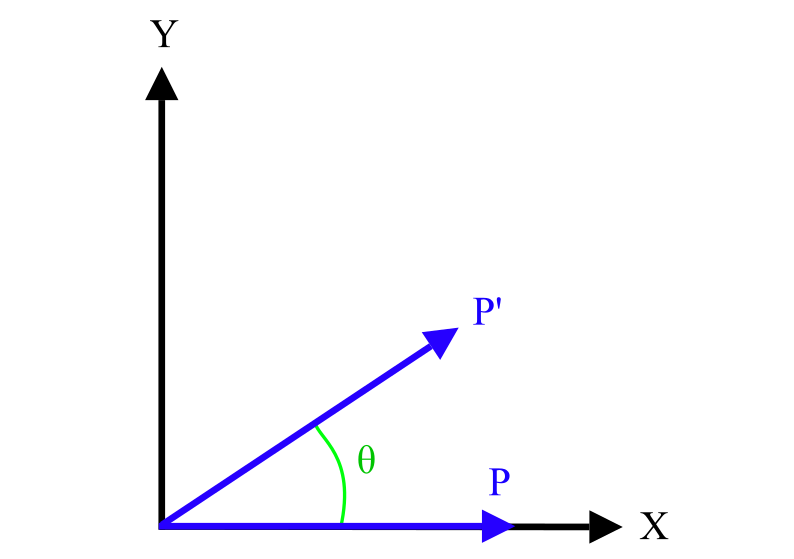
\includegraphics[width=0.4\textwidth]{figs/rotation.pdf}
\caption{Application of the rotation matrix}
\label{fig:rotation}
\end{figure}

\section{Coordinate systems}
To deal with abstract geometric objects, it is often easier to work in different coordinate systems. For example, a cell of a grid, displayed on a standard monitor may be defined in terms of grid coordinates or screen-pixel coordinates. To convert between the two systems, translation functions are required. Equation \ref{eq:gtos} translates grid coordinates to screen coordinates, whereas equation \ref{eq:stog} translates screen coordinates to grid coordinates. \(S\) and \(G\) denote the screen and grid coordinate systems respectively. The subscripts \(w\) and \(h\) denote the respective width and height of each coordinate system.

\begin{equation} \label{eq:gtos}
S_{x, y} = G_{x, y} \; / \; G_{w, h} \times S_{w, h}
\end{equation}

\begin{equation} \label{eq:stog}
G_{x, y} = S_{x, y} \; / \; S_{w, h} \times G_{w, h}
\end{equation}

\section{Set comprehension}
Set comprehension is a method of defining a set by stating the conditions that elements within the set must satisfy. The set \{1, 2, 3\} is described by equation \ref{eq:comprehension}. The first term denotes the superset from which to derive elements. The second term denotes the conditions that must be met for elements to appear in the set.

\begin{equation} \label{eq:comprehension}
S = \left\{x \in \mathbb{Z} : 1 \leq x \leq 3 \right\}
\end{equation}

The semi-colon delimiter is used if there are several conditions that must be met for elements to appear in the set. For example, the set \{1, 3\} may be described by equation \ref{eq:conditions}.

\begin{equation} \label{eq:conditions}
S = \left\{x \in \mathbb{Z} : 1 \leq x \leq 3 ; x \neq 2 \right\}
\end{equation}

Set comprehension may be used as an effective method for describing infinite sets, such as equation \ref{eq:inf1} for the set of integers greater than three, or equation \ref{eq:inf2} for the set of rational numbers between zero and one.

\begin{equation} \label{eq:inf1}
S = \left\{x \in \mathbb{Z} : x > 3 \right\}
\end{equation}

\begin{equation} \label{eq:inf2}
S = \left\{x \in \mathbb{R} : 0 < x < 1 \right\}
\end{equation}

\section{Inverse tangent}
The arctan2 function is a variation on the arctangent function that is used when the direction of a rotation around the origin is important. The standard arctangent function's range of principal values is limited from \(-\pi / 2\) to \(\pi / 2\). To calculate inverse tangents that span all four quadrants, the arctan2 function is required. It is defined in equation \ref{eq:arctan2}.

\begin{equation} \label{eq:arctan2}
\text{atan2}(y, x) =
\begin{cases}
\text{atan}(y / x) & x > 0 \\
\pi + \text{atan}(y / x) & y \geq 0, x < 0 \\
-\pi + \text{atan}(y / x) & y < 0, x < 0 \\
\pi / 2 & y > 0, x = 0 \\
-\pi / 2 & y < 0, x = 0 \\
\text{undefined} & y = 0, x = 0
\end{cases}
\end{equation}

% Simulation environment
\chapter{Simulation environment}
\clearpage

\section{Obstacles}
\label{sec:obstacles}
Obstacles are represented within the simulation as a list of polygons, each containing at least three vertices. The environment class is responsible for maintaining this list, as well as defining the width and height of the simulation environment. The ordering of vertices within each obstacle is important. Starting from an arbitrary vertex, successive vertices must track the perimeter of the obstacle in either a clockwise or anti-clockwise direction. Figure \ref{fig:env1} shows an example environment constructed from a set of obstacles.

\begin{figure}[h]
\centering
\includegraphics[width=0.65\textwidth]{figs/env1.png}
\caption{An example environment constructed from obstacles. The blue obstacle also serves as a beacon entity, explained in section \ref{sec:kalman}.}
\label{fig:env1a}
\end{figure}

\begin{figure}[h]
\centering
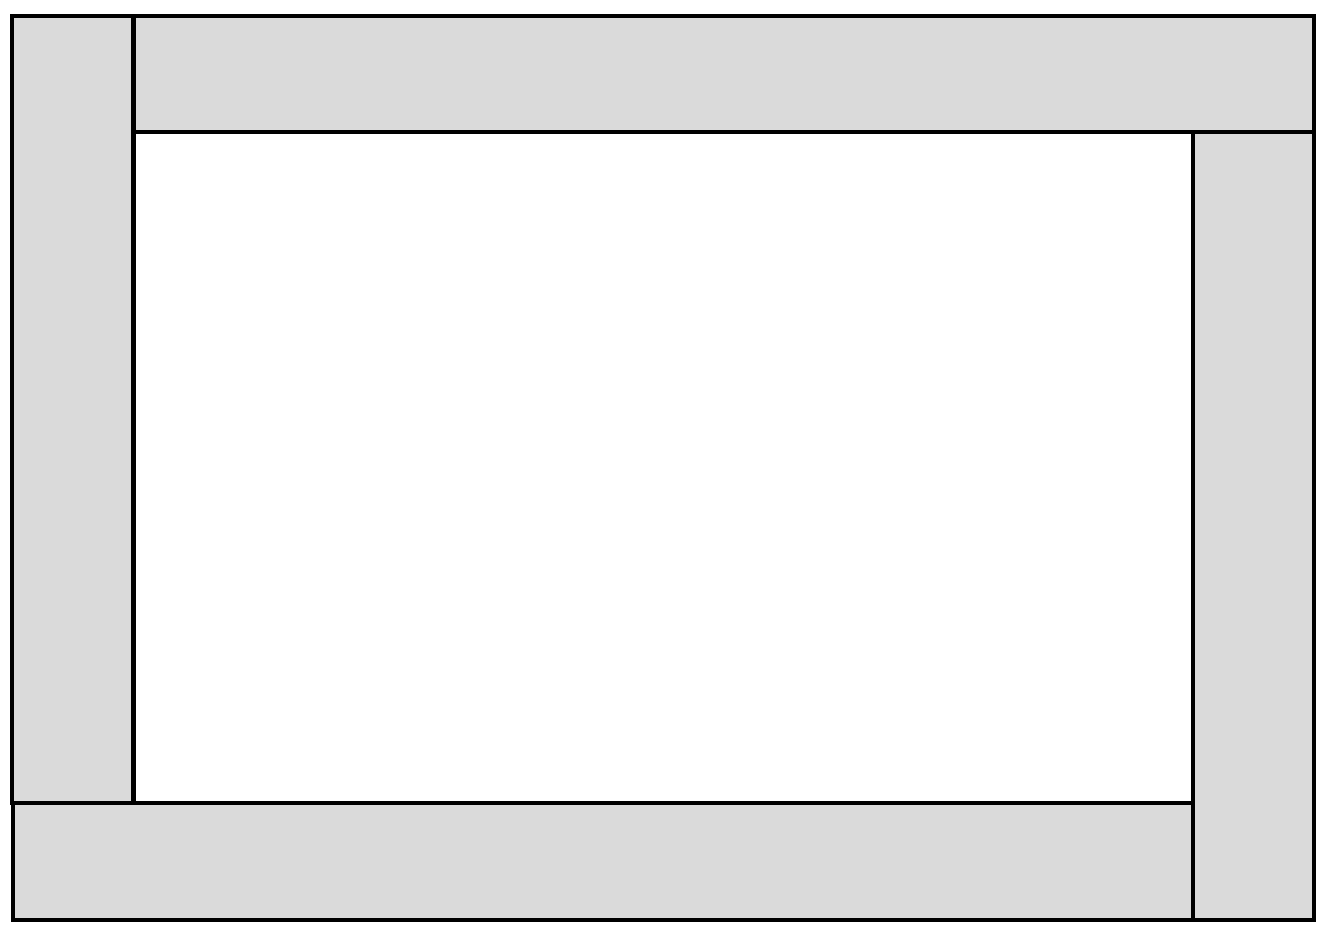
\includegraphics[width=0.4\textwidth]{figs/walls.pdf}
\caption{Generalising walls as obstacles}
\label{fig:walls}
\end{figure}

The walls of the simulation are represented by four additional polygons placed within the environment on construction, shown in figure \ref{fig:walls}. This means that the same drawing and obstacle evaluation functions may be used, instead of handling walls separately. There is no limitation on where obstacles may be placed; they can overlap, be contained within each other and be placed partially out-of-bounds, if required. These kinds of redundancies have a negligible effect on the efficiency of the simulation and may help to simplify the environment creation process for the user.	

\section{Robot} \label{sec:robot}
The robot class is used to represent the robot within the simulation environment. Static properties of the robot, such as width, height and movement rates, are passed into the constructor and an application programming interface is provided containing the basic operations to control the robot. These basic operations modify the dynamic properties of the robot, such as current location and angular direction. Gaussian white noise is applied on robot movements to promote the isomorphism between the simulated robot and a real-world equivalent.

	\subsection{API} \label{sec:api}
The robot's API consists of four operations; forward, backward, left and right. Each operation takes a parameter of type float, which is the amount that the robot has been requested to move (or turn). The actual amount moved by the robot is susceptible to Gaussian white noise, which is generated using the Box-Muller method.

To preserve proportionality, the amount requested to move is multiplied by the static noise value to determine the variance of the noise function, shown in equation \ref{eq:noise}. The symbol \(r\) denotes the amount that the robot is requested to move and \(\eta\) denotes the static noise level within the system. Finally, the application of the homogeneous translation matrix, shown in equation \ref{eq:movement}, determines the new location of the robot in the case of forward and backwards movement and simple angular addition is used in the case of left and right turns.

\begin{samepage}
\begin{equation} \label{eq:noise}
D \sim N(r, \eta \times r)
\end{equation}

\begin{equation} \label{eq:movement}
\begin{pmatrix} x^{'} \\ y^{'} \\ 1 \end{pmatrix} = rand(D)
\begin{pmatrix}
1 & 0 & cos \theta \\
0 & 1 & sin \theta \\
0 & 0 & 1
\end{pmatrix}
\begin{pmatrix} x \\ y \\ 1 \end{pmatrix}
\end{equation}
\end{samepage}
	
	\subsection{Collision handling} \label{sec:collision}
In a real-world situation, robots may not intersect obstacles. To simulate this phenomenon, some basic collision handling functionality is built into the robot class \cite{ericson05}. After each movement, the function `updateVertices' is called, which re-calculates the corner coordinates of the robot. The function `updateCollision' checks whether any of the vertices of the robot are within an obstacle or any vertices of an obstacle are within the robot. If they are, then the move is reversed. Figure \ref{fig:collisions} demonstrates some of the possible cases for collision between the robot and an obstacle.

\begin{figure}[h]
  \centering
  \subfloat[One vertex collision]{\label{fig:collision1}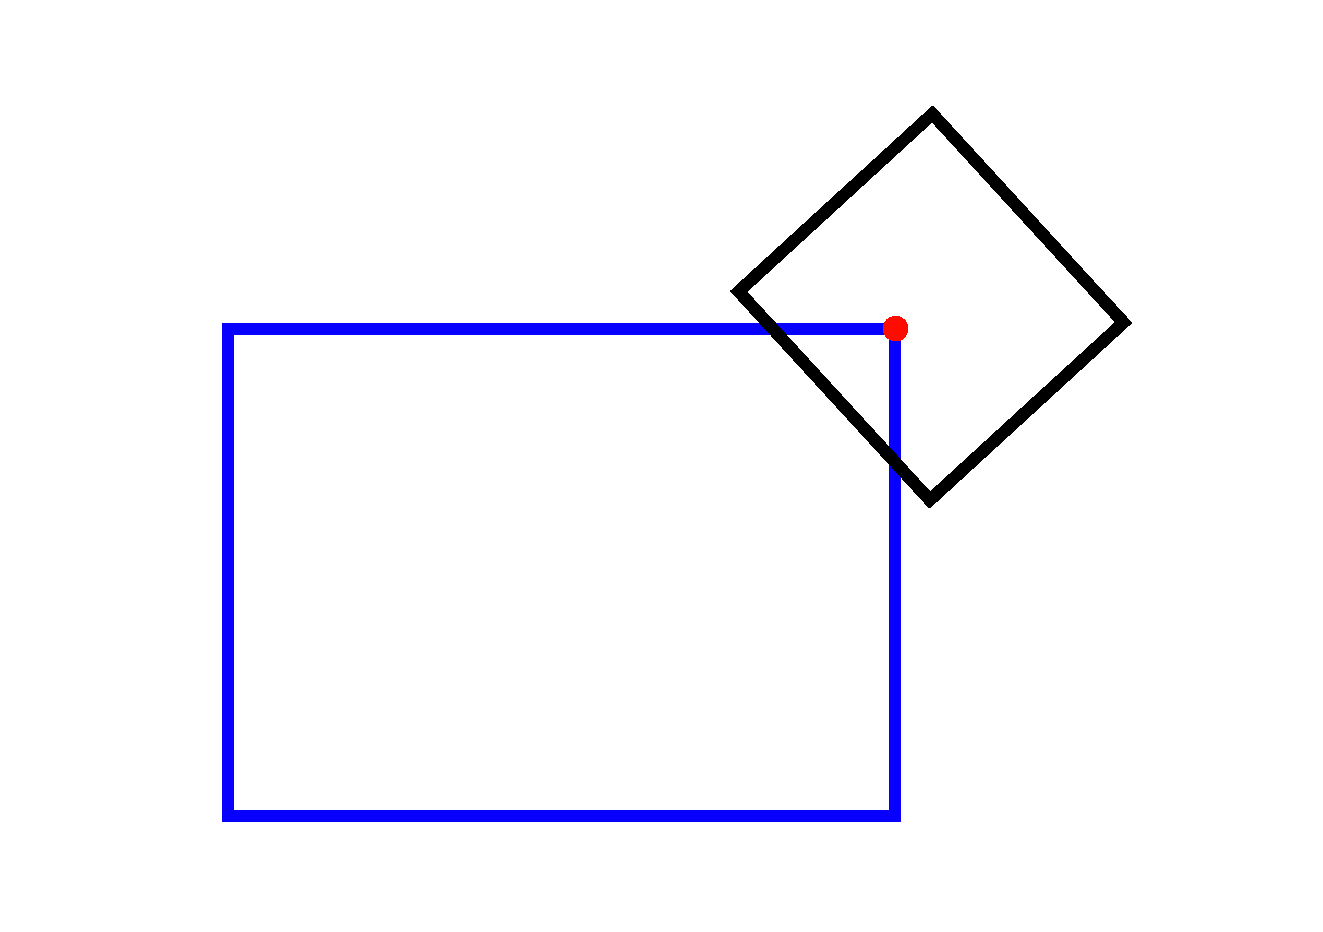
\includegraphics[width=0.3\textwidth]{figs/collision1.pdf}}                
  \subfloat[One vertex collision]{\label{fig:collision2}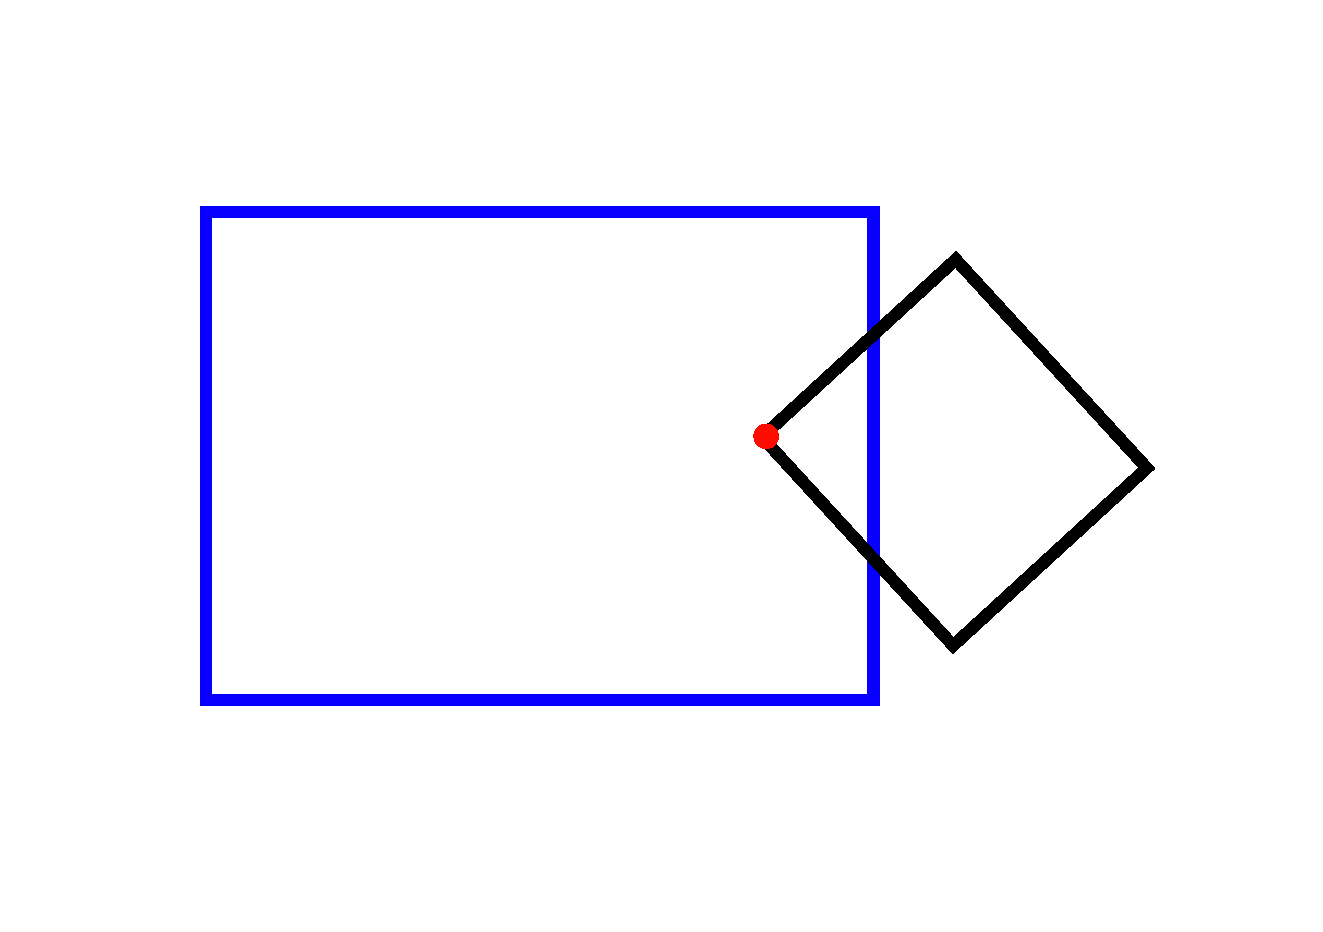
\includegraphics[width=0.3\textwidth]{figs/collision2.pdf}}
  \subfloat[Two vertex collisions]{\label{fig:collision3}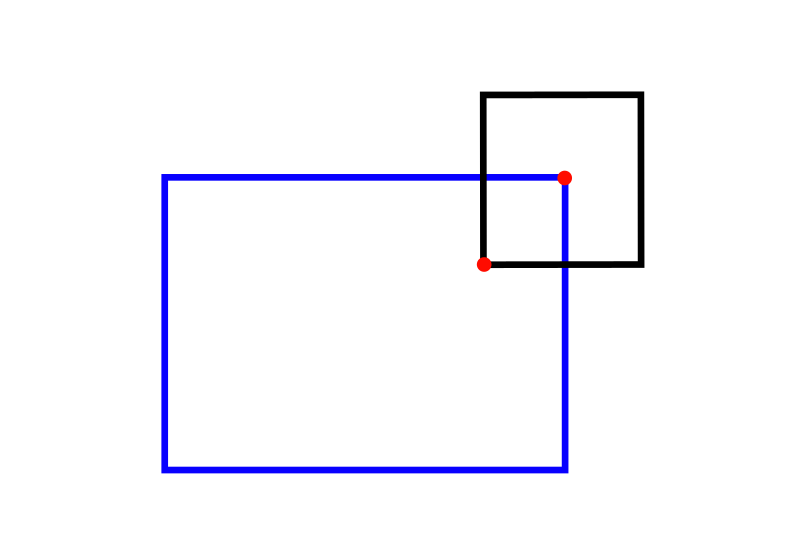
\includegraphics[width=0.3\textwidth]{figs/collision3.pdf}}
  \caption{Some possible cases for collision between the robot and an obstacle}
  \label{fig:collisions}
\end{figure}
	
\section{Detector} \label{sec:detector}
The `lidar' function in the robot class is responsible for updating the angular direction of the detector. This simply carries out angular addition, but also takes into account turns of the robot, as it would in a real-world scenario. The `updateLidar' function is responsible for calculating the point at which the detector intersects with an obstacle \cite{ehrich09}. When returning from this function, the value that is set, corresponds to the distance from the robot to the intercept and does not contain information concerning the obstacle or vertex of intersection.

A hill-climbing approach is implemented to determine the distance of the intersection \cite{russell03}. The vertices of each obstacle are iterated over and every edge combination is passed to the `lidarIntercept' function. This returns the vertex of the intersection between the detector and the current edge if one exists. The lidar distance is set to the nearest vertex returned from the `lidarIntercept' function.

	\subsection{Intersections} \label{sec:intersections}
To determine where the intersection occurs, the equation of the line for the object detector and the current edge are calculated. For there to be a valid intersection point, three criteria must be met. The first criterion is that the lines must not be parallel- in this case, a check can be made that the determinant of the two equations is not equal to zero. Secondly, the intersection must lie within the bounds of the edge. Finally, the intersection must lie on the correct side of the robot, corresponding to the emmision direction of the object detector.

\section{Behaviour}
The behaviour class takes low level sensory data and transforms it into more useful complex representations that may later be used by the explorative strategies. It carries out multi-dimensional Kalman filtering on the expected location of the robot as an attempt to localise itself. It maintains a grid representation of the environment and provides a framework for explorative strategies to query potential collisions.

	\subsection{Kalman filter} \label{sec:kalman}
\label{sec:kalman}
As the robot moves around its environment, uncertainty as to the location of the robot gradually builds due to the Gaussian white noise contained within the system. This in turn causes degradation of the robot's understanding of its environment. The behaviour class tracks this uncertainty in the form of covariance in the x and y planes. Any obstacle may be set as a `beacon' entity, which the robot may use to localise itself \cite{maybeck79}.

		\subsubsection{Prediction}
When a beacon is detected, the behaviour class sets its current location to the robot's actual location within the environment. The current covariance is set to zero and the Kalman prediction process begins. A multi-dimensional array holds data about the previous moves of the robot. This is iterated over backwards until a previous measurement with zero covariance is found. On each iteration, an estimation is made as to the robot's location, by backtracking from the newly discovered certain location. The covariance as to the uncertainty of this reverse path is also tracked, which may then be used to combine the sensory results into an improved understanding of the robot's path.

		\subsubsection{Correction}
The Kalman correction process calculates the improved location and covariance for each iteration by combining corresponding points on the original, forwards path, and the predicted backwards path. Equations \ref{eq:kalmanx1} and \ref{eq:kalmany1} are calculated to estimate the new location based on the ratio of certainty between each pairing. The pairs (\(x1, y1\)) and (\(x2, y2\)) denote the location vectors on the forwards and backwards paths, whilst the pairs (\(\sigma_{x1}^{2}, \sigma_{y1}^{2}\)) and (\(\sigma_{x2}^{2}, \sigma_{y2}^{2}\)) denote the covariances associated with those locations. Equations \ref{eq:kalmanx2} and \ref{eq:kalmany2} are used to calculate the covariance for the new location. This will always be less than that of the minimum input covariances, hence the robot's \emph{understanding} of its path is improved.

\begin{samepage}
\begin{equation} \label{eq:kalmanx1}
\mu_{x} = [\sigma_{x2}^{2} / (\sigma_{x1}^{2} + \sigma_{x2}^{2})]x1 + [\sigma_{x1}^{2} / (\sigma_{x1}^{2} + \sigma_{x2}^{2})]x2
\end{equation}

\begin{equation} \label{eq:kalmany1}
\mu_{y} = [\sigma_{y2}^{2} / (\sigma_{y1}^{2} + \sigma_{y2}^{2})]y1 + [\sigma_{y1}^{2} / (\sigma_{y1}^{2} + \sigma_{y2}^{2})]y2
\end{equation}

\begin{equation} \label{eq:kalmanx2}
1 / \sigma_{x}^{2} = (1 / \sigma_{x1}^{2}) + (1 / \sigma_{x2}^{2})
\end{equation}

\begin{equation} \label{eq:kalmany2}
1 / \sigma_{y}^{2} = (1 / \sigma_{y1}^{2}) + (1 / \sigma_{y2}^{2})
\end{equation}
\end{samepage}

	\subsection{Grid model} \label{sec:grid}
The grid model is a high level construct primarily designed to be used by the explorative strategies as a tool for reasoning about their current understanding of the environment. It assumes no prior knowledge and dynamically resizes and rescales in accordance with configurable criteria. Figure \ref{fig:gridmodel} shows an instance of the grid model constructed from the environment shown in figure \ref{fig:env1a}.

Functionality is provided for mapping points onto the grid and translating between \emph{world} and grid coordinates. Special consideration is made for compatibility with Kalman filtering to ensure that the grid model is a true representation of the updated sensory data, after a correction process has occurred. Mechanisms for feedback are built into the grid in the form of `completeness' and `accuracy' which may be tracked throughout the simulation.

\begin{figure}[h]
\centering
\includegraphics[width=0.65\textwidth]{figs/gridmodel.png}
\caption{An instance of the grid model}
\label{fig:gridmodel}
\end{figure}

		\subsubsection{Mapping points}

To map a point on the grid, the location and covariance of the point are passed as parameters to the `mapPoint' function. A bounding box is calculated that determines over which cells to iterate. Theoretically, every cell in the grid should be reconsidered due to the unbounded characteristic of the Normal distribution, but in practice, this is not necessary. The bounding box is limited to three standard deviations from the mean, covering approximately 99.9\% of possible obstacle locations, and is considerably more efficient than a calculatory census of grid cells. For each cell within the bounding box, the probability that the obstacle measurement lies within the cell is calculated. If the calculated probability exceeds the existing probability then the value is replaced.

To calculate the probability, the normal distributions are set up for the x and y planes, shown in equations \ref{eq:normalx} and \ref{eq:normaly} respectively. The mean parameter for each distribution is the relevant component of the location passed to the function. These distributions are then used to calculate the probability that the obstacle lies in the subsection of each independent plane by differencing of the relevant cumulative distribution functions- equations \ref{eq:px} and \ref{eq:py}. The \(w\) in the equations refers to a translation function that maps grid-cell coordinates to `world' coordinates. These independent probabilities are multiplied together to gain the overall probability that the obstacle measurement lies within the current cell, shown in equation \ref{eq:pxy}. This is equivalent to finding the probability of the intersection of the two areas, shown in figure \ref{fig:subsection}.

\begin{samepage}
\begin{equation} \label{eq:normalx}
X \sim N(\mu_{x}, \sigma_{x}^2)
\end{equation}

\begin{equation} \label{eq:normaly}
Y \sim N(\mu_{y}, \sigma_{y}^2)
\end{equation}

\begin{equation} \label{eq:px}
P_{x} = P(x < w(C_{x} + 1)) - P(x < w(C_{x}))
\end{equation}

\begin{equation} \label{eq:py}
P_{y} = P(y < w(C_{y} + 1)) - P(y < w(C_{y}))
\end{equation}

\begin{equation} \label{eq:pxy}
P_{x, y} = P_{x} \times P_{y}
\end{equation}
\end{samepage}

\begin{figure}[h]
\centering
\includegraphics[width=0.8\textwidth]{figs/grid_subsection.png}
\caption{Calculating the probability that a measurement occurred in an arbitrary cell by finding the intersection of areas in orthogonal planes, for a grid mapped onto a bivariate Normal distribution}
\label{fig:subsection}
\end{figure}	
		
		\subsubsection{Dynamics} \label{sec:dynamics}
The dimensions of the grid are determined by the points it has been requested to map. After the bounding box has been calculated, the `mapPoint' function checks whether the box is fully contained within the grid. If it is not, then a resize process takes place. The cardinality of the two-dimensional `cells' array is increased, and all prior points are remapped. The resize operation has a time complexity of \(O(n)\), where \(n\) is the number of points previously mapped to the grid. Resize operations tend to take place frequently at the start of the simulation and rarely as it progresses. Therefore, the time spent resizing the grid has a minimal impact on the runtime of the simulation.

Rescaling the grid is a little more complex. As configuration for the simulation, three parameters are set; `start granularity', `minimum granularity' and `split determinant'. The size of each cell within the grid is initially set to the start granularity. After a point has been mapped to a cell, a check is carried out on its direct neighbours, including diagonals. If the probability of the current cell and any neighbouring cell is above the split determinant then the `divide' function is called. This halves the current granularity and remaps the points within the grid. Rescaling the grid is a costly operation. Therefore, setting a minimum granularity ensures that the grid does not rescale indefinitely.

		\subsubsection{Kalman compatibility} \label{sec:kc}
After a Kalman correction process has occurred, many of the points that had been mapped to the grid will have changed. To ensure the grid is a true representation based on the sensory data, these points need to be remapped. This is not as simple as working the `mapPoint' function in reverse, as the `max' operand for combining the probabilities on a cell is non-commutative. A naive approach, would be simply to remap every point. This would be hugely inefficient as only a few points change between updates. Instead, an internalised stack is maintained within the grid class, that keeps track of changes since a previous Kalman update. Prior to the correction process, the grid is reverted back to its previous state by popping all changes. The modified points are then mapped to the grid.
		
		\subsubsection{Feedback}
As a tool for the evaluation of explorative strategies, functions to measure `completeness' and `accuracy' are provided as part of the grid class. Completeness is calculated by counting the number of non-zero cells and dividing this summation by the total number of cells. Accuracy is calculated by finding the mean probability of all non-zero cells. The general idea is that the completeness metric gives a comparative value for an explorative strategy's overall coverage of the grid, whereas the accuracy metric refers to its certainty of the representation.

	\subsection{Collision detection}
A collision detection module is built into the behaviour class that may be used by the explorative strategies, to query the probability that a given move will result in collision \cite{millington07}. The `overlay' function estimates the corner coordinates of the robot, given a location and angular direction, and returns the set of grid cells that the robot would overlap.

Overlays are retrieved in the `collision' function for the current location of the robot and its estimated location, after the given move takes place. The set complement of the estimated location cells in the current location cells is determined, shown in equation \ref{eq:complement}. The summation of the probabilities of the cells contained within the complement set is calculated. By clamping this value to one, a slight performance gain can be achieved by exiting from the function early with the same results, shown in equation \ref{eq:summation}.

\begin{samepage}
\begin{equation} \label{eq:complement}
S_{\Delta} = S_{\beta} - S_{\alpha}
\end{equation}

\begin{equation} \label{eq:summation}
\min \left( \sum_{i \in S_{\Delta}} i, 1 \right)
\end{equation}
\end{samepage}
	
\section{Graph window} \label{sec:graph}
The graph window plots completeness and accuracy throughout the simulation. The relevant functions are polled every second and plotted to the graph. Polling is a better solution than re-plotting on each simulation update, due to the complexities of the functions. The x-axis rescales constantly such that the data is spread maximally, for better viewing. The graph is generated in pure OpenGL using a mixture of lines, text and colours, shown in figure \ref{fig:graph}.

\begin{figure}[h]
\centering
\includegraphics[width=0.9\textwidth]{figs/graph.png}
\caption{The graph window}
\label{fig:graph}
\end{figure}

\section{Configuration} \label{sec:configuration}
To set up the simulation, a bespoke configuration file is read. An XML reader library aggregates the data from this file and passes it to the relevant functions. The configurable elements are split into four sections; `environment', `robot', `behaviour' and `display'. The environment section is used to set up the width and height of the simulation and to define all obstacles and beacons within the environment. The robot section is used to set up the static properties of the robot, such as width, height, move rate and noise. The behaviour section defines the identifier of the explorative strategy to run, as well as the granularity parameters for the grid. Finally, the display section sets up the window dimensions and the default viewing elements, such as the robot path display or the grid model.

	\subsection{XML / DTD}
The configuration file is an XML file that complies with a custom document type definition. XML is a widely used markup language that is well supported. It may be edited in a basic text editor and is human readable. The DTD is provided at the top of all configuration files and serves as a reference for the structure of the XML. Appendix listing \ref{lst:dtd} shows the Document Type Definition used for all configuration files.

	\subsection{Automation} \label{sec:automation}
Additional support for the automation of testing is built into the configuration file. A `runtime' parameter may be set in addition to a `tests' parameter. If there are remaining tests, the simulation will restart when the runtime has elapsed. After each test completes, a text file is appended with the final values for completeness and accuracy. If the robot becomes stuck, that particular test instance will exit early, and the time of exit will also be written to file. This means that software may be left for an extended duration to carry out testing without any additional human interaction.

\newpage
\section{Unit testing}
	\subsection{Robot movements}
Listing \ref{lst:unit1} demonstrates a unit test investigating robot movements. It uses textual outputs liberally to track the behaviour of variables at intermediate stages throughout the function. \\

%%%%%%%%%%%%%%%%%%%%%
\begin{lstlisting}[label=lst:unit1, caption=Carrying out unit testing for robot movements]
/*

Unit test 4/18
Checks that forwards movement works as expected
Revision 1
15/03/11

*/
//Moves the robot unless there is a collision.
void Robot::forward(float amount) {
	cout << "Trying to move by " << amount << " units" << endl;
	
	amount = gaussianRandom(amount, amount * mNoise);
	
	cout << "After noise is applied: " << amount << endl;
	
	float radians = angle * (float)PI / 180;
	
	cout << "Current location: " << location.x << ", " << location.y << endl;
	
	location.x += amount * cos(radians);
	location.y += amount * sin(radians);
	
	cout << "New location:" << location.x << ", " << location.y << endl;
	
	updateVertices();
	updateCollision();

	if (collision) {
		cout << "A collision has occurred, reverting move" << endl;
		
		location.x -= amount * cos(radians);
		location.y -= amount * sin(radians);
		
		cout << "Final location: " << location.x << ", " << location.y;
	}
	updateVertices();
	updateCollision();
}
\end{lstlisting}
%%%%%%%%%%%%%%%%%%%%%

\newpage
	\subsection{Window resizing}
Listing \ref{lst:unit2} demonstrates a unit test for window resizing. The aspects for the window and model are compared and different outputs are generated based on the program flow.\\

%%%%%%%%%%%%%%%%%%%%%
\begin{lstlisting}[label=lst:unit2, caption=Carrying out unit testing for window resizing]
/*

Unit test 7/18
Checks that window resizing works correctly
Revision 1
17/03/11

*/
//Called when the window is reshaped. Maintains aspect ratio.
void reshapeCallback(int width, int height) {
	cout << "Window dimensions: " << width << ", " << height << endl;
	
	double windowAspect = (double)width / height;
	double modelAspect = (double)DisplayE->width / DisplayE->height;
	double offset;
	
	cout << "wAspect: " << windowAspect << ", mAspect: " << modelAspect << endl;

	if (modelAspect > windowAspect) {
		cout << "model aspect is greater";
		
		offset = (1 - windowAspect / modelAspect) * height;
		
		xFrom = 0; xTo = width;
		yFrom = offset / 2; yTo = height - yFrom;
	}
	else {
		cout << "window aspect is greater";
		
		offset = (1 - modelAspect / windowAspect) * width;
		
		xFrom = offset / 2; xTo = width - xFrom;
		yFrom = 0; yTo = height;
	}
	
	cout << "Setting viewport to (" << xFrom << ", " << yFrom << ", " << xTo - xFrom << ", " << yTo - yFrom;
	
	glViewport(xFrom, yFrom, xTo - xFrom, yTo - yFrom);
}
\end{lstlisting}
%%%%%%%%%%%%%%%%%%%%%

\newpage
	\subsection{Kalman filtering}
Listing \ref{lst:unit3} demonstrates a unit test to verify the behaviour of the Kalman filter. The covariance is checked for improvement and the size of the `reverse' array is tested after it has been cleared.\\

%%%%%%%%%%%%%%%%%%%%%
\begin{lstlisting}[label=lst:unit3, caption=Carrying out unit testing for Kalman filtering]
/*

Unit test 12/18
Checks that the Kalman filter is working correctly
Revision 2
24/03/11

*/
//Calculate best estimate locations based on variance weightings.
for (unsigned int r = 1, d = data.size() - 2; r < reverse.size(); r++, d--) {
	//Mean location.
	float x = data[d].x + (data[d].xV / (data[d].xV + reverse[r].xV)) * (reverse[r].x - data[d].x);
	float y = data[d].y + (data[d].yV / (data[d].yV + reverse[r].yV)) * (reverse[r].y - data[d].y);
	
	cout << "Averaged " << x << ", " << y;
	cout << " from " << data[d].x << ", " << data[d].y << " and ";
	cout << reverse[r].x << ", " << reverse[r].y << endl;

	//Improved variance.
	float xVar = data[d].xV * reverse[r].xV / (data[d].xV + reverse[r].xV);
	float yVar = data[d].yV * reverse[r].yV / (data[d].yV + reverse[r].yV);
	
	if (xVar > data[d].xV || xVar > reverse[r].xV) cout << "Error: x variance has not improved" << endl;
	if (yVar > data[d].yV || yVar > reverse[r].yV) cout << "Error: y variance has not improved" << endl;

	//Update the data records.
	data[d].x = x;
	data[d].y = y;
	data[d].xV = xVar;
	data[d].yV = yVar;

	cout << "Attempting to map point..." << endl;
	
	//Map the improved points to grid.
	Vertex v = getVertex(data[d].x, data[d].y, data[d].l, data[d].d);
	grid.mapPoint(v.x, v.y, data[d].xV, data[d].yV, true);
	
	cout << "Point mapped";
}
reverse.clear();
if (reverse.size() != 0) cout << "Error: reverse contains left over elements";
\end{lstlisting}
%%%%%%%%%%%%%%%%%%%%%

\newpage
\section{Acceptance testing}
\begin{enumerate}
\item The simulation must be able to represent environments of varying dimensions. This requirement is met successfully, see sections \ref{sec:obstacles} and \ref{sec:configuration}. The user is able to set the dimensions of the model in the configuration file which are passed to the environment constructor.

\item Environments must have the capability to store a list of obstacles. This requirement is met successfully, see section \ref{sec:obstacles}. The environment class contains a member variable that is a list of obstacles, where each obstacle is a list of vertices.

\item The software must simulate a robot within the obstructed environment, with an API that may be used by each explorative strategy. This requirement is met successfully, see sections \ref{sec:robot} and \ref{sec:api}. A robot is simulated within the environment with an API consisting of four basic operations; forwards, backwards, left and right.

\item Additive white Gaussian noise must be applied on each robot movement. This requirement is met successfully, see section \ref{sec:api}. Noise is generated using the Box-Muller transform and applied on each movement. The noise is scaled according to its magnitude, preserving proportionality and ensuring it is additive.

\item Collisions must be handled appropriately such that the robot may not intersect objects. This requirement is met successfully, see section \ref{sec:collision}. If any of the robot's vertices are contained within an obstacle, or vice versa, the move is reversed.

\item An object-detector must be simulated that measures the distance to the nearest obstacle at a give angle. This requirement is met successfully, see sections \ref{sec:detector} and \ref{sec:intersections}. The `updateLidar' function calculates the distance to the nearest obstacle.

\item The behavioural module must attempt to compensate for noise within the system. This requirement is met successfully, see section \ref{sec:kalman}. A two-dimensional Kalman filter is implemented that calculates improved estimates for the robot's previous locations.

\item An internalised representation of the environment must be maintained for the robot. This requirement is met successfully, see section \ref{sec:grid}. The grid model is created and updated with sensory measurements which the robot may use as a high level construct for reasoning about its environment.

\item The robot must be able to interface with different strategies for exploring the environment. This requirement is met successfully, see section \ref{sec:configuration}. The configuration file is used to specify which strategy to run, which is passed to the `runStrategy' function inside the behaviour module.

\item When the simulation window is resized, its aspect ratio must be the same. This requirement is met successfully, see listing \ref{lst:unit2}. The window and model aspect ratios are compared and the viewport is set appropriately \cite{angel09}.

\item A graph window must be displayed showing the current progress of each explorative strategy. This requirement is met successfully, see section \ref{sec:graph}. The completeness and accuracy functions for the grid are polled each second and plotted to a graph.

\item The simulation must be able to use a configuration file to load environments and configure many aspects of the system. This requirement is met successfully, see section \ref{sec:configuration}. A wide array of elements are configurable, such as static robot values, obstacle locations and the current exploration strategy.

\item The capability to automate testing must be provided as part of the configuration file. This requirement is met successfully, see section \ref{sec:automation}. The `runtime' and `tests' values are set in the configuration file. When the runtime expires, a new test begins until all tests are complete.

\item The simulation must provide the capability to toggle different data elements to be displayed. This requirement is met successfully, see section \ref{sec:automation}. The default view elements can be set in the configuration file and then toggled from a right click menu as the simulation runs. Shortcut keys are also provided for toggling each view.

\item The user must be able to pause the simulation at any time and toggle the current display elements. This requirement is met successfully. The space bar key may be used to pause the simulation or by going through the right-click menu. Viewing elements may be changed as usual, in this state.

\item The simulation should run at near real-time speed. The complexity of its underlying operations should support this requirement. This requirement is met successfully, see section \ref{sec:dynamics}. The complexity of the resize, rescale and kalman update operations are optimised to allow for the simulation to run at near real-time speeds.

\item The simulation should be frame-rate independent. This requirement is met successfully, see section \ref{sec:opengl}. The OpenGL framework is used which allows control over the frame and animation rates \cite{ruiter08}.

\item The system should be object-oriented for purposes of extensibility and reuse. This requirement is met successfully, see section \ref{sec:hier}. The system is divided into different objects shown in the class hierarchy diagram. Classes may be members of, or contain references to other classes.

\item The software code should be well-commented such that it is accessible to other developers. This requirement is met successfully, see listings \ref{lst:unit1}, \ref{lst:unit2} and \ref{lst:unit3}. The software code is commented and presented appropriately.

\item The explorative strategies should be sufficiently decoupled such that they may be modified with ease. This requirement is met successfully, see chapter \ref{sec:strats} and section \ref{sec:configuration}. The current strategy may be specified in the configuration file. To modify a strategy, the relevant case statement in the `runStrategy' function is altered.
\end{enumerate}

\chapter{Exploration strategies} \label{sec:strats}
\clearpage

\section{Wall following}
Wall following is frequently used as an algorithm for maze solving. When applied to an open environment, it may still provide good coverage \cite{brooks87} \cite{webb09}. The wall following algorithm uses the grid model and begins by calculating the equation of the line that passes through the front-right corner of the robot at a 45 degree angle, equation \ref{eq:followline}. \(P\) denotes the location of the front-right corner and \(\theta\) denotes the angular direction.

\begin{equation} \label{eq:followline}
y = tan(\theta - 45)x + (P_{y} - tan(\theta - 45) \times P_{x})
\end{equation}

The next stage implements a Digital Differential Analyser, shown in figure \ref{fig:dda}. This involves stepping along the line in x and y, and adding all cells that intersect with the line to a set. The cell that contains the front-right corner of the robot determines where to begin stepping. The direction to step in x and y is determined by the direction of the ray emitting from the front-right corner and is shown by the orange arrows in the diagram.

\begin{figure}[h]
\centering
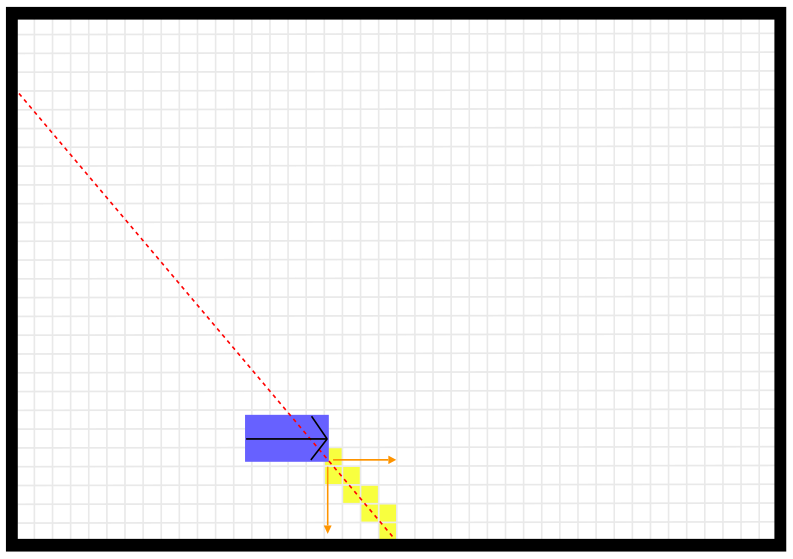
\includegraphics[width=0.8\textwidth]{figs/wallfollow.pdf}
\caption{The implementation of a Digital Differential Analyser to determine which cells intersect a ray emitting from the front-right corner of the robot}
\label{fig:dda}
\end{figure}

For every cell in the set, the distance from its centre to the robot's location is calculated, if its grid probability is greater than zero, shown in equations \ref{eq:nonzeroset} and \ref{eq:mindist}. \(S\) denotes the set of cells to consider and \(r\) denotes the robot's location. All cells that are further from the robot than the non-zero cell with minimum distance are removed from the set, for the purposes of displaying a unique view related to the wall following strategy.

\begin{samepage}
\begin{equation} \label{eq:nonzeroset}
\beta = \{c \in S : c_{p} \neq 0\}
\end{equation}

\begin{equation} \label{eq:mindist}
d = \min \left(\sqrt{(c_{x} - r_{x})^{2} + (c_{y} - r_{y})^{2}} \right), \quad \forall c \in \beta
\end{equation}
\end{samepage}

	\subsection{Controlling distance}
The minimum distance from the wall is defined as one width of the robot, whereas the maximum distance from the wall is defined as two widths of the robot. If the value of \(d\) is less than the minimum then it turns away from the wall. If \(d\) is greater than the maximum then it turns towards the wall. Otherwise, the robot continues forwards.

Moves are alternated between forwards and turning so that the robot moves in arcs rather than turning on the spot. This prevents the robot from endlessly rotating when too far or too close to the wall. Figure \ref{fig:s1path} shows an example run of the wall following strategy after 30 seconds. The green line represents the robot's path.

\begin{figure}[h]
\centering
\includegraphics[width=0.65\textwidth]{figs/s1path.png}
\caption{The robot's path, shown in green, after a 30 second run of the wall following strategy. The `tracker' overlay is enabled, displaying the set of cells, derived from the digital differential analyser, up to the first non-zero cell.}
\label{fig:s1path}
\end{figure}

	\subsection{Collisions and cycles}
Collision prevention and cycle detection are built into the strategy. On each forward movement, the strategy queries the probability of collision using the detection function contained within the behaviour class. If this probability is greater than zero, the forwards movement is skipped and the robot continues to turn. To prevent cycles, the previous move is tracked. The strategy may not choose a move for the current turn that undoes the move from the previous turn. This constraint is shown in equation \ref{eq:difmove}.

\begin{equation} \label{eq:difmove}
move(t) \not= \neg move(t - 1), \quad t > 1
\end{equation}

\newpage
\section{Random avoidance}
The random avoidance strategy instructs the robot to travel in a straight line until it is about to collide. It will then turn a random distance and continue to travel forwards. This strategy tends to explore further into the centre of the environment than the wall following strategy so, in theory, should gain better coverage. It uses the collision detection function to query when it is about to collide based on the grid model. If the robot becomes stuck, it will attempt to move in any direction that it has not been previously tried for the current move, as an attempt to free itself. Figure \ref{fig:s2path} shows an example run of the random avoidance strategy after 30 seconds.

\begin{figure}[h]
\centering
\includegraphics[width=0.65\textwidth]{figs/s2path.png}
\caption{The robot's path, shown in green, after a 30 second run of the random avoidance strategy}
\label{fig:s2path}
\end{figure}

A cyclic problem arises with this strategy if the robot becomes stuck and backwards is selected as the valid move to free itself. The next move the robot will attempt is forwards. This will lock the robot into a forwards-backwards cycle and no explorative progress will be made. To counter this problem, a flag is set to true if the previous move was backwards. This may then be checked on the successive move. If it is true then the robot will not choose to move forwards.

A slightly more complicated problem arises related to the random direction for turning. If the robot collides again shortly after it has turned away from the wall, it may choose the opposite direction in which to turn. This is inefficient as the robot will spend most of its time backtracking over areas it has already explored. To counter this problem, a `remaining' variable is maintained. When a new turning direction is chosen, the remaining value is set to two lengths of the robot. If it collides again before it has travelled the distance stored in the remaining variable, then it will choose to turn in the same direction.

\newpage
\section{Direct quadrants}
The direct quadrants strategy attempts to build on the random avoidance strategy by directing the robot towards unexplored areas. An additional abstract data structure is maintained, containing the number of turns the robot has spent in different sections of the simulation environment. This data structure may then be used to direct the robot towards quadrants with fewer turns. It uses the same collision handling and cycle prevention as the random avoidance strategy, based on the grid model.

Equation \ref{eq:curquad} is used to calculate in which quadrant the robot is located. \(w^{'}\) denotes a function that maps world coordinates to grid-cell coordinates, \(Q_{w}\) and \(Q_{h}\) denote the dimensions of the quadrant data structure and \(G_{w}\) and \(G_{h}\) denote the dimensions of the grid model. Initially, the number of turns that the robot has spent in the current quadrant is incremented, shown in equation \ref{eq:quadincr}.

\begin{equation} \label{eq:curquad}
\begin{pmatrix} x \\ y \end{pmatrix} =
\begin{pmatrix}
\lfloor w^{'}(r_{x}) \times Q_{w} \; / \; G_{w} \rfloor \\
\lfloor w^{'}(r_{y}) \times Q_{h} \; / \; G_{h} \rfloor
\end{pmatrix}
\end{equation}

\begin{equation} \label{eq:quadincr}
Q_{x, y} = Q_{x, y} + 1
\end{equation}

	\subsection{Second ordering}
The direct neighbour with the minimum turns determines the next quadrant to navigate towards. When the robot is located in a boundary quadrant, the choice of neighbours is reduced. If more than one neighbour has the minimum number of turns, a second ordering is required. The set containing the centres of the neighbours with the minimum turns is constructed, shown in equation \ref{eq:mincentres}. \(M\) denotes the set of neighbours with minimum turns.

The set containing the unit vectors from the robot's location to the centres of the quadrants with minimum turns is constructed, shown in equation \ref{eq:vectorcentres}. The angular offsets from the robot's current heading are calculated for each unit vector- equation \ref{eq:minoffset}, and the quadrant corresponding to the minimal offset is chosen. This means that the time spent turning towards quadrants will be minimised, improving the efficiency of the strategy. Figure \ref{fig:directquad} demonstrates the quadrant selection process.

\begin{samepage}
\begin{equation} \label{eq:mincentres}
C = \left\{ c :
\begin{pmatrix} c_{x} \\ c_{y} \end{pmatrix} =
\begin{pmatrix}
w((m_{x} + 0.5) \times G_{w} \; / \; Q_{w}) \\
w((m_{y} + 0.5) \times G_{h} \; / \; Q_{h})
\end{pmatrix}
; \; m \in M \right\}
\end{equation}

\begin{equation} \label{eq:vectorcentres}
U = \left\{ \overset{\rightarrow}{u} :
\begin{pmatrix} u_{x} \\ u_{y} \end{pmatrix} =
\widehat{\begin{pmatrix}
c_{x} - r_{x} \\ c_{y} - r_{y}
\end{pmatrix}}
; \; c \in C \right\}
\end{equation}

\begin{equation} \label{eq:minoffset}
\alpha = \min (\arctan_{2}(\sin \theta, \cos \theta) - \arctan_{2}(u_{y}, u_{x})), \quad \forall u \in U
\end{equation}
\end{samepage}

The `turn' flag is set to false if \(\alpha\) is within an acceptable range, otherwise it is true. The `turnLeft' flag is set to true if \(\alpha\) is between 180 and 360 degrees, otherwise it is false. These flags are used within the random avoidance strategy as a form of encapsulation. If `turn' is true, the robot will turn on the spot, in the direction determined by the `turnLeft' flag, instead of moving forwards by default. Figure \ref{fig:s3path} shows an example run of the direct quadrants strategy.

\newpage
\begin{figure}[t]
\centering
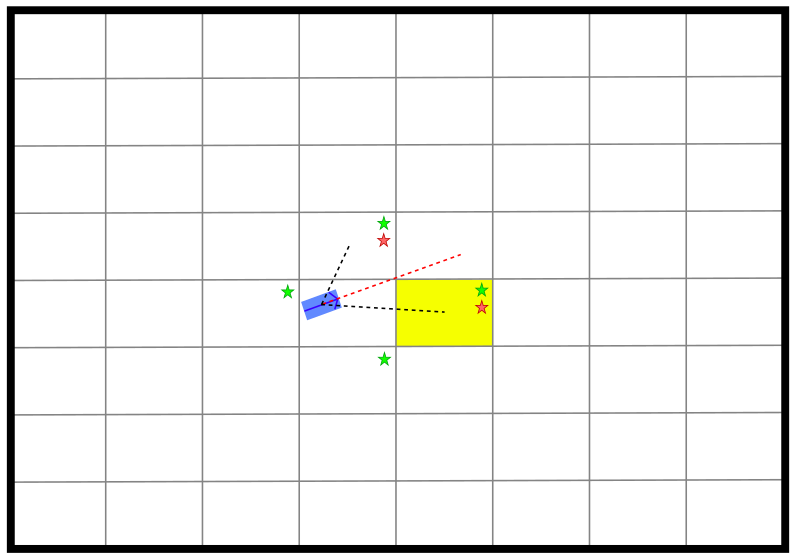
\includegraphics[width=0.8\textwidth]{figs/directquad.pdf}
\caption{An example selection process of the direct quadrants strategy. Green stars denote neighbour quadrants, red stars denote neighbour quadrants with minimal turns, the shaded quadrant is selected.}
\label{fig:directquad}
\end{figure}

\begin{figure}[b]
\centering
\includegraphics[width=0.65\textwidth]{figs/s3path.png}
\caption{The robot's path, shown in green, after a 30 second run of the direct quadrants strategy. The quadrant overlay is enabled displaying the neighbouring cells the strategy is considering. The grey line denotes the vector to the selected quadrant.}
\label{fig:s3path}
\end{figure}
\clearpage

\section{Implied quadrants}
The need for a modification of the direct quadrants strategy is demonstrated in figure \ref{fig:repeatedcollision}. When an obstacle spans many quadrants, the robot will tend to attempt to head towards the quadrants on the other side of the obstacle. With the direct quadrants strategy, the robot has a fixed understanding of where it wants to go and turns to face that direction. Therefore, the strategy will constantly direct the robot into the wall and trigger the collision prevention code. Usually, the robot will get round the obstacle due to the `remaining' variable as part of the collision prevention, but it is somewhat inefficient.

The implied quadrants strategy builds upon direct quadrants, but alternates between forwards and turning movements. Additionally, the second ordering criterion for selecting quadrants is different. When there is more than one quadrant with a minimum number of turns, the quadrant that is nearest to the robot's location is selected. In the case of figure \ref{fig:repeatedcollision}, the robot will still attempt to head towards the quadrant on the other side, but it has more flexibility in its pathing.

\begin{figure}[h]
\centering
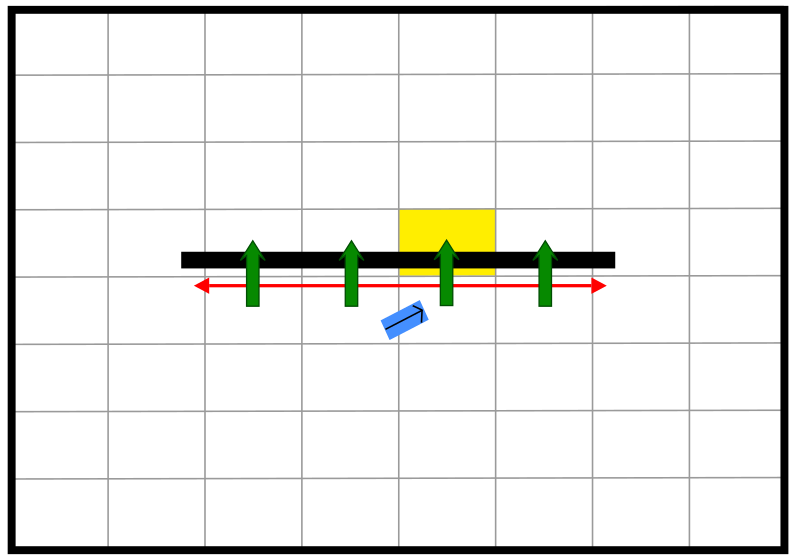
\includegraphics[width=0.8\textwidth]{figs/repeatedcollision.pdf}
\caption{A demonstration of a problem that arises with the direct quadrants strategy. The green arrows denote the direction the strategy chooses for the cells under the obstacle. The red arrow denotes the path that is likely to be repeated by the robot, causing inefficiency.}
\label{fig:repeatedcollision}
\end{figure}

	\subsection{Second ordering}
The minimum distance from the robot's location to the centres of the cells with minimum turns, is calculated, shown in equation \ref{eq:impliedsecond}. The quadrant corresponding to the minimum is selected. Figure \ref{fig:impliedquad} demonstrates the difference in quadrant selection. Figure \ref{fig:s4path} shows an example run of the implied quadrants strategy.

\begin{equation} \label{eq:impliedsecond}
d = \min \left(\sqrt{(c_{x} - r_{x})^{2} + (c_{y} - r_{y})^{2}}\right), \quad\forall c \in C
\end{equation}

\newpage
\begin{figure}[t]
\centering
\includegraphics[width=0.8\textwidth]{figs/impliedquad.pdf}
\caption{An example selection process of the implied quadrants strategy. Green stars denote neighbour quadrants, red stars denote neighbour quadrants with minimal turns, the shaded quadrant is selected.}
\label{fig:impliedquad}
\end{figure}

\begin{figure}[b]
\centering
\includegraphics[width=0.65\textwidth]{figs/s4path.png}
\caption{The robot's path, shown in green, after a 30 second run of the implied quadrants strategy. The quadrant overlay is enabled displaying the neighbouring cells the strategy is considering. They grey line denotes the vector to the selected quadrant.}
\label{fig:s4path}
\end{figure}
\clearpage

% Empirical evaluation
\chapter{Empirical evaluation} \label{sec:ee}
\clearpage

\section{Test environments}
Three environments have been created to test how well the strategies perform in different scenarios. Test environment one, figure \ref{fig:env1}, is fifty units in width and height. It is a relatively open environment and has a beacon entity located centrally.

\begin{figure}[h]
\centering
\includegraphics[width=0.55\textwidth]{figs/env1.png}
\caption{Test environment one}
\label{fig:env1}
\end{figure}

Test environment two, figure \ref{fig:env2}, is far more occluded and contains more areas without direct line of sight to a beacon obstacle. It has the same dimensions as test environment one.

\begin{figure}[h]
\centering
\includegraphics[width=0.55\textwidth]{figs/env2.png}
\caption{Test environment two}
\label{fig:env2}
\end{figure}
\clearpage

Test environment three, figure \ref{fig:env3}, is much larger, containing roughly twice the area of the other environments. It is seventy units in width and height and has a greater number of areas in which the robot could potentially become immobilised. There are two beacon entities located relatively central.

\begin{figure}[h]
\centering
\includegraphics[width=0.55\textwidth]{figs/env3.png}
\caption{Test environment three}
\label{fig:env3}
\end{figure}

\section{Collecting results}
The automated testing routines built into the configuration file are used to collect results. A test configuration file is created for each strategy on each environment. The length of time the strategies may explore each environment is set to two minutes. This is a long enough time for the robot to get round each environment multiple times. On the other hand, it is not too long such that the strategies can explore every environment in huge amounts of detail. The number of tests is set to one hundred for each configuration file, but this can be increased if the results are inconclusive \cite{hastie08}. This equates to forty machine hours to collect results, assuming that each strategy runs at real-time speeds, shown in equation \ref{eq:timespent}.

\begin{equation} \label{eq:timespent}
120 \; \text{seconds} \times 100 \; \text{tests} \times 4\; \text{strategies} \times 3\; \text{environments} = 40 \; \text{hours}
\end{equation}

\section{Early exits}
One apparent criterion for rating the performance of strategies is how frequently they cause the robot to become stuck. Figure \ref{fig:earlyexits} shows the number of tests that did not reach the end of their two minute time. Figure \ref{fig:earlytime} shows the average early exit times for each environment and strategy.

\newpage
\begin{figure}[t]
\centering
\vspace{-130pt}
\includegraphics[width=0.9\textwidth]{figs/earlyexits_bar.pdf}
\vspace{-130pt}
\caption{A bar chart showing the number of tests that exited early due to the robot getting stuck, for each strategy and environment}
\label{fig:earlyexits}
\end{figure}

\begin{figure}[b]
\centering
\vspace{-130pt}
\includegraphics[width=0.9\textwidth]{figs/earlytime_bar.pdf}
\vspace{-130pt}
\caption{A bar chart showing the average time that the robot became stuck, for each strategy and environment}
\label{fig:earlytime}
\end{figure}
\clearpage

\newpage
\section{Completeness vs. accuracy}
	\subsection{Environment one}
Figure \ref{fig:scat1} shows the completeness and accuracy results for test environment one. Table \ref{tab:e1_stats} shows many statistical properties of the data sets corresponding to environment one. The table has been coloured to show the strategy rankings for each criteria. Wall following has the highest mean completeness and accuracy, but gets stuck more frequently and earlier than the implied quadrants strategy. The direct quadrants strategy performed the worst for almost all criteria.
	
\begin{figure}[h]
\centering
\vspace{-150pt}
\includegraphics[width=\textwidth]{figs/e1_scatter.pdf}
\vspace{-150pt}
\caption{Environment one's scatter graph, plotting completeness vs. accuracy for each strategy}
\label{fig:scat1}
\end{figure}

\definecolor{r1}{rgb}{0.75, 1, 0.75}
\definecolor{r2}{rgb}{1, 1, 0.75}
\definecolor{r3}{rgb}{1, 0.875, 0.75}
\definecolor{r4}{rgb}{1, 0.75, 0.75}
\begin{table}[h]
\begin{tabular}{| l | c | c | c | c |}
\hline
& Wall following & Random avoidance & Direct quadrants & Implied quadrants \\ \hline
\(C_{\mu}\) & \cellcolor{r1} 0.2982 & \cellcolor{r3} 0.2805 & \cellcolor{r4} 0.2747 & \cellcolor{r2} 0.2874 \\ \hline
\(C_{\sigma^{2}}\) & \cellcolor{r2} 0.0025 & \cellcolor{r1} 0.0024 & \cellcolor{r4} 0.0036 & \cellcolor{r3} 0.0029 \\ \hline
\(A_{\mu}\) & \cellcolor{r1} 0.8082 & \cellcolor{r2} 0.7838 & \cellcolor{r4} 0.7523 & \cellcolor{r3} 0.7726 \\ \hline
\(A_{\sigma^{2}}\) & \cellcolor{r1} 0.00042703 & \cellcolor{r2} 0.00091907 & \cellcolor{r4} 0.0022 & \cellcolor{r3} 0.0011 \\ \hline
\(E_{\mu}\) & \cellcolor{r4} 42.0143 & \cellcolor{r2} 47.6528 & \cellcolor{r3} 47.1826 & \cellcolor{r1} 50.425 \\ \hline
\(E_{\%}\) & \cellcolor{r2} 0.1 & \cellcolor{r3} 0.11 & \cellcolor{r4} 0.2 & \cellcolor{r1} 0.09 \\ \hline
\end{tabular}
\caption{Environment one, strategy statistics. The elements in the far left column are: completeness mean, completeness variance, accuracy mean, accuracy variance, early exit time mean, amount of early exits.}
\label{tab:e1_stats}
\end{table}
\clearpage

\newpage
	\subsection{Environment two}
Figure \ref{fig:scat2} shows the completeness and accuracy results for test environment one. Table \ref{tab:e2_stats} shows many statistical properties of the data sets corresponding to environment one. The table has been coloured to show the strategy rankings for each criteria. The implied quadrants strategy came out on top, performing the best for almost all criteria. The wall following strategy was the worst whilst the random avoidance and direct quadrants strategies came out about even. The direct quadrants and implied quadrants are tied for first place for the mean completeness.
	
\begin{figure}[h]
\centering
\vspace{-150pt}
\includegraphics[width=\textwidth]{figs/e2_scatter.pdf}
\vspace{-150pt}
\caption{Environment two's scatter graph, plotting completeness vs. accuracy for each strategy}
\label{fig:scat2}
\end{figure}

\begin{table}[h]
\begin{tabular}{| l | c | c | c | c |}
\hline
& Wall following & Random avoidance & Direct quadrants & Implied quadrants \\ \hline
\(C_{\mu}\) & \cellcolor{r4} 0.1703 & \cellcolor{r3} 0.1992 & \cellcolor{r1} 0.2708 & \cellcolor{r1} 0.2708 \\ \hline
\(C_{\sigma^{2}}\) & \cellcolor{r3} 0.105 & \cellcolor{r1} 0.0071 & \cellcolor{r4} 0.123 & \cellcolor{r2} 0.0095 \\ \hline
\(A_{\mu}\) & \cellcolor{r3} 0.7743 & \cellcolor{r4} 0.7674 & \cellcolor{r2} 0.7903 & \cellcolor{r1} 0.7967 \\ \hline
\(A_{\sigma^{2}}\) & \cellcolor{r4} 0.0087 & \cellcolor{r2} 0.0034 & \cellcolor{r3} 0.0042 & \cellcolor{r1} 0.0026 \\ \hline
\(E_{\mu}\) & \cellcolor{r4} 17.0862 & \cellcolor{r3} 48.2655 & \cellcolor{r2} 51.1066 & \cellcolor{r1} 60.6272 \\ \hline
\(E_{\%}\) & \cellcolor{r2} 0.36 & \cellcolor{r3} 0.37 & \cellcolor{r3} 0.37 & \cellcolor{r1} 0.32 \\ \hline
\end{tabular}
\caption{Environment two, strategy statistics. The elements in the far left column are: completeness mean, completeness variance, accuracy mean, accuracy variance, early exit time mean, amount of early exits.}
\label{tab:e2_stats}
\end{table}
\clearpage

\newpage
	\subsection{Environment three}
Figure \ref{fig:scat3} shows the completeness and accuracy results for test environment one. Table \ref{tab:e3_stats} shows many statistical properties of the data sets corresponding to environment one. The table has been coloured to show the strategy rankings for each criteria. The random avoidance strategy performed the best, followed closely by the direct quadrants strategy. The wall following strategy collected the most accurate data, but was the least complete, whereas the direct quadrants strategy collected the most complete data, but was the least accurate.
	
\begin{figure}[h]
\centering
\vspace{-150pt}
\includegraphics[width=\textwidth]{figs/e3_scatter.pdf}
\vspace{-150pt}
\caption{Environment three's scatter graph, plotting completeness vs. accuracy for each strategy}
\label{fig:scat3}
\end{figure}

\begin{table}[h]
\begin{tabular}{| l | c | c | c | c |}
\hline
& Wall following & Random avoidance & Direct quadrants & Implied quadrants \\ \hline
\(C_{\mu}\) & \cellcolor{r4} 0.071 & \cellcolor{r2} 0.1156 & \cellcolor{r1} 0.1189 & \cellcolor{r3} 0.1017 \\ \hline
\(C_{\sigma^{2}}\) & \cellcolor{r3} 0.0015 & \cellcolor{r2} 0.0012 & \cellcolor{r1} 0.001 & \cellcolor{r4} 0.0019 \\ \hline
\(A_{\mu}\) & \cellcolor{r1} 0.7855 & \cellcolor{r2} 0.7739 & \cellcolor{r4} 0.7423 & \cellcolor{r3} 0.7516 \\ \hline
\(A_{\sigma^{2}}\) & \cellcolor{r2} 0.0021 & \cellcolor{r2} 0.0021 & \cellcolor{r1} 0.002 & \cellcolor{r4} 0.004 \\ \hline
\(E_{\mu}\) & \cellcolor{r4} 23.2453 & \cellcolor{r1} 72.3422 & \cellcolor{r2} 64.6144 & \cellcolor{r3} 45.6485 \\ \hline
\(E_{\%}\) & \cellcolor{r4} 0.8 & \cellcolor{r1} 0.33 & \cellcolor{r3} 0.52 & \cellcolor{r2} 0.35 \\ \hline
\end{tabular}
\caption{Environment three, strategy statistics. The elements in the far left column are: completeness mean, completeness variance, accuracy mean, accuracy variance, early exit time mean, amount of early exits.}
\label{tab:e3_stats}
\end{table}
\clearpage

\subsection{Combined environments}
Figure \ref{fig:scat123} shows the completeness and accuracy results for the combined environment data. Table \ref{tab:combined_stats} shows many statistical properties of the combined data sets. The table has been coloured to show the strategy rankings for each criteria. The wall following strategy performed the worst for all criteria except the average accuracy, for which it excelled considerably. The random avoidance strategy has minimal variances, but did not do well for the average completeness and accuracy values.  The implied quadrants strategy was complete, but lacked accuracy. The implied quadrants strategy is the least likely to become stuck.

\begin{figure}[h]
\centering
\vspace{-150pt}
\includegraphics[width=\textwidth]{figs/e123_scatter.pdf}
\vspace{-150pt}
\caption{Combined environment scatter graph, plotting completeness vs. accuracy for each strategy}
\label{fig:scat123}
\end{figure}

\begin{table}[h]
\begin{tabular}{| l | c | c | c | c |}
\hline
& Wall following & Random avoidance & Direct quadrants & Implied quadrants \\ \hline
\(C_{\mu}\) & \cellcolor{r4} 0.1798 & \cellcolor{r3} 0.1984 & \cellcolor{r1} 0.2215 & \cellcolor{r2} 0.22 \\ \hline
\(C_{\sigma^{2}}\) & \cellcolor{r4} 0.0135 & \cellcolor{r1} 0.0081 & \cellcolor{r2} 0.0109 & \cellcolor{r3} 0.0118 \\ \hline
\(A_{\mu}\) & \cellcolor{r1} 0.7893 & \cellcolor{r2} 0.775 & \cellcolor{r4} 0.7617 & \cellcolor{r3} 0.7736 \\ \hline
\(A_{\sigma^{2}}\) & \cellcolor{r4} 0.0039 & \cellcolor{r1} 0.0022 & \cellcolor{r3} 0.0032 & \cellcolor{r2} 0.0029 \\ \hline
\(E_{\mu}\) & \cellcolor{r4} 22.9752 & \cellcolor{r1} 57.9913 & \cellcolor{r2} 56.8307 & \cellcolor{r3} 52.5210 \\ \hline
\(E_{\%}\) & \cellcolor{r4} 0.42 & \cellcolor{r2} 0.27 & \cellcolor{r3} 0.3633 & \cellcolor{r1} 0.2533 \\ \hline
\end{tabular}
\caption{Combined environments, strategy statistics. The elements in the far left column are: completeness mean, completeness variance, accuracy mean, accuracy variance, early exit time mean, amount of early exits.}
\label{tab:combined_stats}
\end{table}
\clearpage

\section{Ranking strategies} \label{sec:ranking}
It is important to consider the performance of each strategy in the context of their intended application \cite{hastie08}. Without prior knowledge of the task, it is difficult to compare the strategies and definitively claim which is the best. Instead, a performance ranking system is created that scores each strategy according to a weighted set of parameters. This means that strategies may be evaluated for suitability to a given task by determining the importance of constituent criteria, relevant to completion of the task.

	\subsection{Parameters}
The parameters for evaluation of strategies are the same as demonstrated in tables \ref{tab:e1_stats} through \ref{tab:combined_stats}. A ranking of first place for a particular category scores one point, second place scores two points, etc. These totals are summed up for each criteria based on the individual environment data, shown in table \ref{tab:scores}. This leads to the scoring matrix, equation \ref{eq:scorematrix}, which may be used to score each strategy's performance for a given application by defining the weighting values of \(C_{u}\), \(C_{\sigma^{2}}\), \(A_{\mu}\), \(A_{\sigma^{2}}\), \(E_{\mu}\) and \(E_{\%}\). It is important to note that the minimum scores are the better performing strategies, whereas the maximum scores are the worst.

\begin{table}[h]
\begin{tabular}{| l | c | c | c | c |}
\hline
& Wall following & Random avoidance & Direct quadrants & Implied quadrants \\ \hline
\(C_{\mu}\) & \cellcolor{r4} 9 & \cellcolor{r3} 8 & \cellcolor{r1} 6 & \cellcolor{r1} 6 \\ \hline
\(C_{\sigma^{2}}\) & \cellcolor{r2} 8 & \cellcolor{r1} 4 & \cellcolor{r3} 9 & \cellcolor{r3} 9 \\ \hline
\(A_{\mu}\) & \cellcolor{r1} 5 & \cellcolor{r3} 8 & \cellcolor{r4} 10 & \cellcolor{r2} 7 \\ \hline
\(A_{\sigma^{2}}\) & \cellcolor{r2} 7 & \cellcolor{r1} 6 & \cellcolor{r3} 8 & \cellcolor{r3} 8 \\ \hline
\(E_{\mu}\) & \cellcolor{r4} 12 & \cellcolor{r2} 6 & \cellcolor{r3} 7 & \cellcolor{r1} 5 \\ \hline
\(E_{\%}\) & \cellcolor{r3} 8 & \cellcolor{r2} 7 & \cellcolor{r4} 10 & \cellcolor{r1} 4 \\ \hline
\end{tabular}
\caption{The summation of scores for each criteria and strategy from the individual environment data. The elements in the far left column are: completeness mean, completeness variance, accuracy mean, accuracy variance, early exit time mean, amount of early exits.}
\label{tab:scores}
\end{table}

\begin{equation} \label{eq:scorematrix}
\begin{pmatrix}
Score(\text{Wall following}) \\
Score(\text{Random avoidance}) \\
Score(\text{Direct quadrants}) \\
Score(\text{Implied quadrants})
\end{pmatrix} =
\begin{pmatrix}
9 & 8 & 5 & 7 & 12 & 8 \\
8 & 4 & 8 & 6 & 6 & 7 \\
6 & 9 & 10 & 8 & 7 & 10 \\
6 & 9 & 7 & 8 & 5 & 4
\end{pmatrix}
\begin{pmatrix} C_{\mu} \\ C_{\sigma^{2}} \\ A_{\mu} \\ A_{\sigma^{2}} \\ E_{\mu} \\ E_{\%} \end{pmatrix}
\end{equation}

\newpage
	\subsection{Example applications} \label{sec:ea}
		\subsubsection{Path finding}
If a robot is assigned to solving the task of path finding, it should attempt to find the shortest path between two points. It may be more efficient for the robot initially to explore the environment before its primary task. The completeness mean and variance criteria are most important for generating an overall understanding as opposed to accuracy which maps smaller areas in greater detail. It is also important that the robot does not become immobilised. The scores are calculated for each strategy based on the estimated weightings matrix, shown in equation \ref{eq:scores1}.
		

\begin{equation} \label{eq:scores1}
\begin{pmatrix} 8.3 \\ 6.4 \\ 8.5 \\ 6.1 \end{pmatrix} =
\begin{pmatrix}
9 & 8 & 5 & 7 & 12 & 8 \\
8 & 4 & 8 & 6 & 6 & 7 \\
6 & 9 & 10 & 8 & 7 & 10 \\
6 & 9 & 7 & 8 & 5 & 4
\end{pmatrix}
\begin{pmatrix} 0.3 \\ 0.3 \\ 0 \\ 0 \\ 0 \\ 0.4 \end{pmatrix}
\end{equation}

With a score of 6.1, the implied quadrants strategy should perform the best. This is closely followed by random avoidance with a score of 6.4. Wall following scores 8.3 and was therefore third, whilst the direct quadrants strategy placed last with a score of 8.5. Therefore, for the application of initial exploration, prior to path finding, the implied quadrants strategy is the better choice.

		\subsubsection{Moving hazardous materials}
If a robot is assigned to solving the task of moving hazardous materials, it's main priority should be not to spill the materials. Spills would most likely be caused by colliding with an obstacle at speed. This is most likely to happen if the robot did not expect the obstacle to lie on its path. Therefore, accuracy is far more important than completeness for this application. If the robot became stuck, it would have failed its task, but this should be of less importance than protecting the environment from the hazardous materials. It is preferable that it should become stuck as late as possible to maximise progress. The scores are calculated for each strategy based on the estimated weightings matrix, shown in equation \ref{eq:scores2}.

\begin{equation} \label{eq:scores2}
\begin{pmatrix} 6.8 \\ 6.9 \\ 8.9 \\ 6.9 \end{pmatrix} =
\begin{pmatrix}
9 & 8 & 5 & 7 & 12 & 8 \\
8 & 4 & 8 & 6 & 6 & 7 \\
6 & 9 & 10 & 8 & 7 & 10 \\
6 & 9 & 7 & 8 & 5 & 4
\end{pmatrix}
\begin{pmatrix} 0 \\ 0 \\ 0.4 \\ 0.4 \\ 0.1 \\ 0.1 \end{pmatrix}
\end{equation}

With a score of 6.8, the wall following strategy should perform the best. The random avoidance and implied quadrants strategies are equally as good for second place, with scores of 6.9. The direct quadrants strategy is, once again, the worst strategy with a score of 8.9. Therefore, the best strategy for the application of moving hazardous materials is wall following.

		\subsubsection{Automated cleaning}
Many robots are used for automated cleaning, such as the Roomba. Similar applications could be for cutting grass, or polishing floors. These robots often have a charging station to return to, therefore, it is important that they do not become stuck whilst carrying out their tasks. If they do become stuck, the time at which they do so is not of great importance as it will still fail its task. Completeness and accuracy are equally important. Completeness is required so that the robot can get around most of the environment. Accuracy is required so that it carries out its task up to the edges of obstacles appropriately. The scores are calculated for each strategy based on the estimated weightings matrix, shown in equation \ref{eq:scores3}.

\begin{equation} \label{eq:scores3}
\begin{pmatrix} 8.1 \\ 6.7 \\ 9 \\ 5.5 \end{pmatrix} =
\begin{pmatrix}
9 & 8 & 5 & 7 & 12 & 8 \\
8 & 4 & 8 & 6 & 6 & 7 \\
6 & 9 & 10 & 8 & 7 & 10 \\
6 & 9 & 7 & 8 & 5 & 4
\end{pmatrix}
\begin{pmatrix} 0.1 \\ 0.1 \\ 0.1 \\ 0.1 \\ 0.1 \\ 0.5 \end{pmatrix}
\end{equation}

With a score of 5.5, the implied quadrants strategy came out on top. The random avoidance strategy came second with a score of 6.7. The wall following strategy came third with a score of 8.1. The direct quadrants strategy came last again, with a score of 9. Therefore, for the application of automated cleaning, the implied quadrants strategy should perform the best.

		\subsubsection{Safety critical repairs}
If a group of robots is assigned the task of repairing some safety critical system, it is important to have a clear understanding of how well the robots will perform. It is hard to judge how many robots to apply to a given area if its results are considerably varied. Therefore, it is arguably better to deploy several poor performing robots than, fewer robots with unpredictable behaviour. Accuracy should be regarded as more important, as the completeness of the environment will be shared amongst the swarm. It does not matter if a robot becomes stuck, because others may take its place and transport it back for repairs. The scores are calculated for each strategy based on the estimated weightings matrix, shown in equation \ref{eq:scores4}.

\begin{equation} \label{eq:scores4}
\begin{pmatrix} 7 \\ 5.6 \\ 8.8 \\ 8.2 \end{pmatrix} =
\begin{pmatrix}
9 & 8 & 5 & 7 & 12 & 8 \\
8 & 4 & 8 & 6 & 6 & 7 \\
6 & 9 & 10 & 8 & 7 & 10 \\
6 & 9 & 7 & 8 & 5 & 4
\end{pmatrix}
\begin{pmatrix} 0 \\ 0.4 \\ 0.2 \\ 0.4 \\ 0 \\ 0 \end{pmatrix}
\end{equation}

With a score of 5.6, the random avoidance strategy came out on top. Wall following placed second with a score of 7. The implied quadrants strategy was third with a score of 8.2 and direct quadrants was the worst performer, with a score of 8.8. Therefore, for the application of safety critical repairs, the random avoidance strategy should perform the best.

% Conclusions
\chapter{Conclusions}
\clearpage

\section{Choosing strategies}
From the evidence gathered in section \ref{sec:ee}, it is apparent that the choice of strategy is not a simple decision. Instead, it requires some analysis of the context in which the strategy is to be applied. For the general case, it may be useful to examine the rankings in performance of each strategy, for the example applications presented in section \ref{sec:ea}. This makes the assumption that the example applications are somewhat representative of real-world scenarios and that their frequency of occurrence is uniform.

If no prior knowledge of the application of the strategies is known, then the implied quadrants strategy should be chosen as this performed the best for the example applications, scoring the highest in all four tests. The random avoidance and wall following strategies each came out on top for one example application. However, the random avoidance strategy ranked above wall following for applications that were won by the implied quadrants strategy. Therefore, in the general case, random avoidance is slightly better than wall following. The direct quadrants strategy performed the worst in every example application, indicating that it should rarely be chosen for exploration.

It seems curious that the two quadrant-based approaches to exploration scored at opposite ends of the spectrum. Intuitively, it would seem that this phenomenon arises due to the strategies' paradigms for exploration. The direct quadrants strategy attempts to travel towards neighbour quadrants, with minimal turns, by rotating on the spot and travelling in straight lines. The implied quadrants strategy alternates between forwards and turning towards the preferred quadrant. This may be perceived as being more relaxed in the context of control over its heading. The direct quadrants strategy is likely to run into more collisions as a result of this behaviour which is supported by the bar chart showing the number of early exists, figure \ref{fig:earlyexits}.

For larger, more occluded environments, the gap in performance between random avoidance and wall following, tends to widen. This is supported by the combination of statistical tables \ref{tab:e1_stats}, \ref{tab:e2_stats} and \ref{tab:e3_stats}. The occlusion in environment two is greater than that of environment one, and environment three is larger than environment two. It seems likely that random avoidance strategy performs better on large, occluded environments because wall following is ultimately flawed in that it rarely ventures into the centre of environments.

The general procedure for choosing a strategy for a known application, involves analysing the task for the importance of constituent criteria. A weightings matrix should be estimated for the application, based on the importance of each criteria. The weightings matrix should be post-multiplied with the score matrix to obtain `performance' scores for each strategy. The strategy with the minimal score should be selected for the given application. To calculate the score matrix for an additional strategy, it should be ranked in terms of each criteria based on statistical comparison with the other strategies. Section \ref{sec:ranking} explains this process in greater detail.

\section{Critical Evaluation}
The validity of the work presented here is dependent upon the realism incorporated into the simulation. The careful application of noise within the system means that it is somewhat representative of a real-world scenario. Basic collision handling is simulated, although this could be made more realistic by considering the momentum and angular direction of the robot on collision \cite{millington07}. Additionally, the robot movements do not take into account acceleration, which would affect robots in the real-world.

One issue to consider, is whether the behavioural module and explorative strategies could be deployed on a micro-controller. The programming language selected for the software was intentionally chosen to simplify the porting of code, as a lot of low-level micro-controllers support C-based languages, see section \ref{sec:langs}. The object-oriented approach to software development means that it is much easier to port specific modules to devices, as they are mostly decoupled from each other.

The behavioural strategies presented here range from simplistic wall following, or random avoidance, to relatively complex quadrant-based approaches. Although the rankings of strategies in various situations are useful for potential application design, the more useful ideas are presented in the process of empirical evaluation, chapter \ref{sec:ee}. It is arguably more useful for application designers to construct their own strategies, and then rate their performance based on the guidelines presented here.

The use of the grid model shows how a high level construct, may be created from simple sensory data, and applied to the field of autonomous exploration. It may not be the best model for the task, but it provides one possible solution. A benefit of using the grid model is that it is finite. It can indefinitely map points and will maintain a fixed size in memory. Intuitively, this is supported by the concepts of information theory, as repeated data does not carry additional information.

The significance of the completeness and accuracy metrics requires consideration. Ideally, they should be entirely independent variables, but in practice this is unrealistic. If accuracy is poor, the number of cells affected by a sensory measurement is large as its covariance causes the bounding box to span more cells. As a consequence the completeness value increases as there are more cells containing non-zero values. It may be more beneficial to calculate the completeness metric based on the sparsity of information over the grid. In practice, the bias in completeness is present for all strategies, so its affects are negligible.

\section{Management account}
The project went to schedule, requiring almost no changes from the initial Gantt chart, see appendix figures \ref{fig:gantt11} through \ref{fig:gantt32}. Extra time was available towards the end of the project to carry out additional software testing. 18 unit tests were carried out, instead of 10. The graph window feature was decided fairly late into the project as an extension to help the user visualise the progress of each strategy as a metric. The time spent implementing this feature would not have been available if it were not for careful time management.

The use of supervisor meetings was incredibly useful throughout the project. They helped to focus the work-flow to ensure the project was on track. They helped to define the scope of the project and decide on the order of implementation for software modules. Additional perspective as to the direction of the project was valuable.

\section{Reflection}
Overall, a great deal was learnt over the duration of the project, in both software development and the field of autonomous exploration in robotics. At the beginning of the project, the testing of strategies was ambiguous. In contrast, the empirical evaluation, chapter \ref{sec:ee} is one of the most formal and precise processes presented as part of this report. For the study of autonomous exploration, the process of evaluation of strategies is arguably, the most significant piece of work presented here.

If the project were repeated, additional realism would be incorporated, with the most emphasis placed on collision handling. A more accurate model for collisions could be supported such that the angular direction and momentum of the robot are considered. Collision detection should have been handled at a much lower level than the grid model for greater success. The most recent points should have had a higher impact on the collision detection as opposed to treating all sensory data uniformly.

If an existing software simulation could have been utilised for the testing of strategies, this would have allowed much longer for strategy development and analysis. However, a suitable simulation could not be located that provided such low level control over noise and collisions within the system. If the time spent creating additional data views had been reallocated, extra time could have been spent developing strategies.

A slight annoyance with the testing stage was the process of automation, for two reasons. The first is that a file must be created for each strategy on each environment. This is wasteful as many of the tests share the same environment. It would have been more efficient to reference another file for the environment in each test configuration, which would reduce the level of redundancy. The second annoyance with automation was that user interaction was required to start each test configuration file for the project. The level of automation could have been improved by implementing a top-level test file containing references to a list of configurations.

If the project were to be developed further, the obvious extension would be to develop new explorative strategies and increase the quantity of testing. Attempts could be made to create a three-dimensional view of the simulation as it runs. This could lead to more interesting views for the simulation data. The usefulness of the grid model could be analysed in greater detail, potentially leading to a formalised approach for building high level constructs that may be used by autonomous exploration. The three-dimensional exploration problem could be considered. A quad-rotor flying robot could be simulated for the three-dimensional case, perhaps using the Kinect as a sensory input device.

% References
\renewcommand\bibname{References}
\begin{thebibliography}{99}

\bibitem{angel09}
E. Angel,
\emph{Interactive Computer Graphics, A Top-Down Approach Using OpenGL},
Pearson Education Inc.,
2009.

\bibitem{box58}
G.E.P Box and M.E Muller,
\emph{A Note on the Generation of Random Normal Deviates},
Statistical Techniques Research Group,
Princeton,
1958.

\bibitem{brooks87}
R.A Brooks,
\emph{Intelligence without Representation},
MIT Artificial Intelligence Laboratory,
Cambridge,
1987.

\bibitem{brooks90}
R.A. Brooks,
\emph{Elephants Don�t Play Chess},
MIT Artificial Intelligence Laboratory,
Cambridge,
1990.

\bibitem{choset05}
H. Choset, K.M. Lynch, S. Hutchinson, G. Kantor, W. Burgard, L.E. Kavraki and S. Thrun,
\emph{Principles of Robot Motion, Theory, Algorithms, and Implementations},
The MIT Press,
Cambridge,
2005.

\bibitem{ehrich09}
R.W. Ehrich,
\emph{2D Liang-Barsky Clipping},
Pixel Education,
2009.\\*
Available: http://goo.gl/E8WwQ

\bibitem{ericson05}
C. Ericson,
\emph{Real Time Collision Detection},
Morgan Kaufman Publishers,
London,
2005.

\bibitem{fowler03}
M. Fowler,
\emph{UML Distilled: A Brief Guide to the Standard Object Modelling Language},
Addison Wesley,
Boston,
2003.

\bibitem{hastie08}
T.Hastie, R. Tibshirani and J. Friedman,
\emph{The Elements of Statistical Learning, Data Mining, Inference, and Prediction},
Springer,
California,
2008.

\bibitem{maybeck79}
P.S. Maybeck,
\emph{Stochastic models, estimation and control},
Academic Press,
New York,
1979.

\bibitem{millington07}
I. Millington,
\emph{Game Physics Engine Development},
Morgan Kaufman Publishers,
London,
2007.

\bibitem{ruiter08}
H.D. Ruiter,
\emph{Frame-Rate Independent Animation using GLUT},
HDR Lab,
2008.\\*
Available: http://goo.gl/DMNi4

\bibitem{russell03}
S.J. Russell and P. Norvig,
\emph{Artificial Intelligence A Modern Approach},
Pearson Education International,
London,
2003.

\bibitem{thrun05}
S. Thrun, W. Burgard and D. Fox,
\emph{Probabilistic Robotics},
The MIT Press,
Cambridge,
2005.

\bibitem{webb09}
B. Webb,
\emph{Animals versus animats: or why not the real iguana?},
School of Informatics,
Edinburgh,
2009.

\end{thebibliography}
\clearpage

% Appendices
\appendix
\chapter*{Appendices}

\begin{lstlisting}[label=lst:dtd, caption=Document Type Definition for the configuration file]
<!DOCTYPE root [
<!ELEMENT root (tests, environment, robot, behaviour, display)>
<!ELEMENT tests (#PCDATA)>
<!ELEMENT environment (polygon*)>
<!ELEMENT polygon (vertex+)>
<!ELEMENT vertex EMPTY>
<!ELEMENT robot (start, moveRate, turnRate, lidarRate, noise)>
<!ELEMENT start (vertex)>
<!ELEMENT moveRate (#PCDATA)>
<!ELEMENT turnRate (#PCDATA)>
<!ELEMENT lidarRate (#PCDATA)>
<!ELEMENT noise (#PCDATA)>
<!ELEMENT behaviour (grid, strategy)>
<!ELEMENT grid (startGran, minGran, split)>
<!ELEMENT startGran (#PCDATA)>
<!ELEMENT minGran (#PCDATA)>
<!ELEMENT split (#PCDATA)>
<!ELEMENT strategy (#PCDATA)>
<!ELEMENT display (default, runtime)>
<!ELEMENT default (robotV?, lidarV?, obstaclesV?, beaconsV?, overlayV?, collisionV?, detectorV?, ellipsesV?, pathV?, gridV?, mappingsV?, verticesV?, trackerV?, debugV?)>
<!ELEMENT robotV EMPTY>
<!ELEMENT lidarV EMPTY>
<!ELEMENT obstaclesV EMPTY>
<!ELEMENT beaconsV EMPTY>
<!ELEMENT overlayV EMPTY>
<!ELEMENT collisionV EMPTY>
<!ELEMENT detectorV EMPTY>
<!ELEMENT ellipsesV EMPTY>
<!ELEMENT pathV EMPTY>
<!ELEMENT gridV EMPTY>
<!ELEMENT mappingssV EMPTY>
<!ELEMENT verticesV EMPTY>
<!ELEMENT trackerV EMPTY>
<!ELEMENT quadrantsV EMPTY>
<!ELEMENT seekV EMPTY>
<!ELEMENT debugV EMPTY>
<!ELEMENT runtime (#PCDATA)>

<!ATTLIST environment width CDATA #REQUIRED>
<!ATTLIST environment height CDATA #REQUIRED>
<!ATTLIST polygon beacon (true|false) 'false'>
<!ATTLIST vertex x CDATA #REQUIRED>
<!ATTLIST vertex y CDATA #REQUIRED>
<!ATTLIST robot width CDATA #REQUIRED>
<!ATTLIST robot height CDATA #REQUIRED>
<!ATTLIST display width CDATA #REQUIRED>
<!ATTLIST display height CDATA #REQUIRED>
]>
\end{lstlisting}

\begin{figure}[h]
\centering
\includegraphics[width=0.9\textwidth]{figs/gantt11.png}
\caption{Initial Gantt chart, page 1}
\label{fig:gantt11}
\end{figure}

\begin{figure}[h]
\centering
\includegraphics[width=0.9\textwidth]{figs/gantt12.png}
\caption{Initial Gantt chart, page 2}
\label{fig:gantt12}
\end{figure}

\begin{figure}[h]
\centering
\includegraphics[width=0.9\textwidth]{figs/gantt21.png}
\caption{Intermediate Gantt chart, page 1}
\label{fig:gantt21}
\end{figure}

\begin{figure}[h]
\centering
\includegraphics[width=0.9\textwidth]{figs/gantt22.png}
\caption{Intermediate Gantt chart, page 2}
\label{fig:gantt22}
\end{figure}

\begin{figure}[h]
\centering
\includegraphics[width=0.9\textwidth]{figs/gantt31.png}
\caption{Final Gantt chart, page 1}
\label{fig:gantt31}
\end{figure}

\begin{figure}[h]
\centering
\includegraphics[width=0.9\textwidth]{figs/gantt32.png}
\caption{Final Gantt chart, page 2}
\label{fig:gantt32}
\end{figure}

\end{document}